% Revised manuscript (rebuilt from the submitted PDF; the original LaTeX source
% and the IEEE Access class file were not available in the repository).
% Every result number is a macro defined in generated/numbers.tex, which is
% written by revision/scripts/05_make_tables.py from the saved predictions.
\documentclass[journal]{IEEEtran}
\usepackage[T1]{fontenc}
\usepackage{amsmath,amssymb}
\usepackage{graphicx}
\usepackage{booktabs}
\usepackage{multirow}
\usepackage{makecell}
\usepackage{threeparttable}
\usepackage{algorithm}
\usepackage{algpseudocode}
\usepackage{xcolor}
\usepackage{tikz}
\usetikzlibrary{arrows.meta,positioning,shapes.geometric,fit,calc}
\usepackage{url}
\usepackage{cite}
\usepackage[hidelinks]{hyperref}

% AUTO-GENERATED by scripts/05_make_tables.py -- do not edit
\newcommand{\AblAsymBayesCost}{0.825}
\newcommand{\AblAsymBayesPrAuc}{0.517}
\newcommand{\AblAsymBayesRecall}{79.8}
\newcommand{\AblAsymBayesRocAuc}{0.572}
\newcommand{\AblAsymBayesSpec}{32.0}
\newcommand{\AblAsymCostCost}{0.625}
\newcommand{\AblAsymCostPrAuc}{0.517}
\newcommand{\AblAsymCostRecall}{94.8}
\newcommand{\AblAsymCostRocAuc}{0.572}
\newcommand{\AblAsymCostSpec}{8.6}
\newcommand{\AblBalBayesCost}{0.890}
\newcommand{\AblBalBayesPrAuc}{0.486}
\newcommand{\AblBalBayesRecall}{76.6}
\newcommand{\AblBalBayesRocAuc}{0.554}
\newcommand{\AblBalBayesSpec}{33.1}
\newcommand{\AblBalCostCost}{0.660}
\newcommand{\AblBalCostPrAuc}{0.486}
\newcommand{\AblBalCostRecall}{94.3}
\newcommand{\AblBalCostRocAuc}{0.554}
\newcommand{\AblBalCostSpec}{4.3}
\newcommand{\AblDoubleBayesCost}{0.903}
\newcommand{\AblDoubleBayesPrAuc}{0.491}
\newcommand{\AblDoubleBayesRecall}{76.9}
\newcommand{\AblDoubleBayesRocAuc}{0.543}
\newcommand{\AblDoubleBayesSpec}{29.8}
\newcommand{\AblDoubleCostCost}{0.681}
\newcommand{\AblDoubleCostPrAuc}{0.491}
\newcommand{\AblDoubleCostRecall}{93.1}
\newcommand{\AblDoubleCostRocAuc}{0.543}
\newcommand{\AblDoubleCostSpec}{5.3}
\newcommand{\AblDuelBayesCost}{0.890}
\newcommand{\AblDuelBayesPrAuc}{0.494}
\newcommand{\AblDuelBayesRecall}{77.3}
\newcommand{\AblDuelBayesRocAuc}{0.559}
\newcommand{\AblDuelBayesSpec}{30.5}
\newcommand{\AblDuelCostCost}{0.644}
\newcommand{\AblDuelCostPrAuc}{0.494}
\newcommand{\AblDuelCostRecall}{94.6}
\newcommand{\AblDuelCostRocAuc}{0.559}
\newcommand{\AblDuelCostSpec}{5.8}
\newcommand{\AblFullBayesCost}{0.864}
\newcommand{\AblFullBayesPrAuc}{0.500}
\newcommand{\AblFullBayesRecall}{79.2}
\newcommand{\AblFullBayesRocAuc}{0.563}
\newcommand{\AblFullBayesSpec}{27.5}
\newcommand{\AblFullCostCost}{0.667}
\newcommand{\AblFullCostPrAuc}{0.500}
\newcommand{\AblFullCostRecall}{93.7}
\newcommand{\AblFullCostRocAuc}{0.563}
\newcommand{\AblFullCostSpec}{5.4}
\newcommand{\AblGammaZeroBayesCost}{0.825}
\newcommand{\AblGammaZeroBayesPrAuc}{0.510}
\newcommand{\AblGammaZeroBayesRecall}{80.6}
\newcommand{\AblGammaZeroBayesRocAuc}{0.576}
\newcommand{\AblGammaZeroBayesSpec}{29.2}
\newcommand{\AblGammaZeroCostCost}{0.645}
\newcommand{\AblGammaZeroCostPrAuc}{0.510}
\newcommand{\AblGammaZeroCostRecall}{94.4}
\newcommand{\AblGammaZeroCostRocAuc}{0.576}
\newcommand{\AblGammaZeroCostSpec}{6.4}
\newcommand{\AblSoftBayesCost}{0.804}
\newcommand{\AblSoftBayesPrAuc}{0.472}
\newcommand{\AblSoftBayesRecall}{82.9}
\newcommand{\AblSoftBayesRocAuc}{0.529}
\newcommand{\AblSoftBayesSpec}{23.5}
\newcommand{\AblSoftCostCost}{0.634}
\newcommand{\AblSoftCostPrAuc}{0.472}
\newcommand{\AblSoftCostRecall}{94.9}
\newcommand{\AblSoftCostRocAuc}{0.529}
\newcommand{\AblSoftCostSpec}{6.5}
\newcommand{\AblWarmBayesCost}{0.896}
\newcommand{\AblWarmBayesPrAuc}{0.497}
\newcommand{\AblWarmBayesRecall}{77.7}
\newcommand{\AblWarmBayesRocAuc}{0.547}
\newcommand{\AblWarmBayesSpec}{27.7}
\newcommand{\AblWarmCostCost}{0.656}
\newcommand{\AblWarmCostPrAuc}{0.497}
\newcommand{\AblWarmCostRecall}{93.8}
\newcommand{\AblWarmCostRocAuc}{0.547}
\newcommand{\AblWarmCostSpec}{7.1}
\newcommand{\AlwaysAcc}{44.2}
\newcommand{\AlwaysAlarm}{100.0}
\newcommand{\AlwaysBalAcc}{50.0}
\newcommand{\AlwaysCost}{0.558}
\newcommand{\AlwaysFN}{0}
\newcommand{\AlwaysFNR}{0.0}
\newcommand{\AlwaysFP}{5,243}
\newcommand{\AlwaysFPR}{100.0}
\newcommand{\AlwaysFone}{61.3}
\newcommand{\AlwaysGmean}{0.0}
\newcommand{\AlwaysMCC}{0.000}
\newcommand{\AlwaysPrec}{44.2}
\newcommand{\AlwaysRecall}{100.0}
\newcommand{\AlwaysSpec}{0.0}
\newcommand{\AlwaysTN}{0}
\newcommand{\AlwaysTP}{4,147}
\newcommand{\AttAucFracSmall}{87}
\newcommand{\AttAucMaxAbsChange}{0.089}
\newcommand{\AttEvasionDropMax}{19}
\newcommand{\AttEvasionDropMin}{4}
\newcommand{\BestBaseline}{RF}
\newcommand{\BestModelAUC}{HGB}
\newcommand{\BestModelCost}{RF}
\newcommand{\CSMLPAttAucMaxDrop}{0.025}
\newcommand{\CSMLPAttAucMaxRise}{0.005}
\newcommand{\CSMLPAttAucaccelspikes}{0.652}
\newcommand{\CSMLPAttAucclean}{0.654}
\newcommand{\CSMLPAttAucfpscap}{0.649}
\newcommand{\CSMLPAttAucrotjitter}{0.654}
\newcommand{\CSMLPAttAucrotsmooth}{0.646}
\newcommand{\CSMLPAttAucspeedscaledown}{0.629}
\newcommand{\CSMLPAttAucspeedscaleup}{0.630}
\newcommand{\CSMLPAttCleanFPR}{93.9}
\newcommand{\CSMLPAttCleanRecall}{99.4}
\newcommand{\CSMLPAttWorstFPR}{100.0}
\newcommand{\CSMLPAttWorstRecall}{95.6}
\newcommand{\CSMLPAttaccelspikesFPR}{99.1}
\newcommand{\CSMLPAttaccelspikesRecall}{99.9}
\newcommand{\CSMLPAttfpscapFPR}{98.3}
\newcommand{\CSMLPAttfpscapRecall}{100.0}
\newcommand{\CSMLPAttrotjitterFPR}{96.5}
\newcommand{\CSMLPAttrotjitterRecall}{99.7}
\newcommand{\CSMLPAttspeedscaleupFPR}{98.2}
\newcommand{\CSMLPAttspeedscaleupRecall}{100.0}
\newcommand{\CSMLPBayesAccEns}{57.4}
\newcommand{\CSMLPBayesAccMean}{57.0}
\newcommand{\CSMLPBayesAccSD}{1.5}
\newcommand{\CSMLPBayesAlarmEns}{73.5}
\newcommand{\CSMLPBayesAlarmMean}{72.1}
\newcommand{\CSMLPBayesAlarmSD}{2.2}
\newcommand{\CSMLPBayesBalAccEns}{60.3}
\newcommand{\CSMLPBayesBalAccMean}{59.7}
\newcommand{\CSMLPBayesBalAccSD}{1.6}
\newcommand{\CSMLPBayesCostEns}{0.691}
\newcommand{\CSMLPBayesCostMean}{0.731}
\newcommand{\CSMLPBayesCostSD}{0.066}
\newcommand{\CSMLPBayesFNEns}{622}
\newcommand{\CSMLPBayesFNMean}{707}
\newcommand{\CSMLPBayesFNREns}{15.0}
\newcommand{\CSMLPBayesFNRMean}{17.0}
\newcommand{\CSMLPBayesFNRSD}{3.1}
\newcommand{\CSMLPBayesFNSD}{129.7}
\newcommand{\CSMLPBayesFPEns}{3,381}
\newcommand{\CSMLPBayesFPMean}{3,332}
\newcommand{\CSMLPBayesFPREns}{64.5}
\newcommand{\CSMLPBayesFPRMean}{63.6}
\newcommand{\CSMLPBayesFPRSD}{2.3}
\newcommand{\CSMLPBayesFPSD}{118.2}
\newcommand{\CSMLPBayesFoneEns}{63.8}
\newcommand{\CSMLPBayesFoneMean}{63.0}
\newcommand{\CSMLPBayesFoneSD}{1.5}
\newcommand{\CSMLPBayesGmeanEns}{54.9}
\newcommand{\CSMLPBayesGmeanMean}{54.9}
\newcommand{\CSMLPBayesGmeanSD}{1.6}
\newcommand{\CSMLPBayesMCCEns}{0.231}
\newcommand{\CSMLPBayesMCCMean}{0.215}
\newcommand{\CSMLPBayesMCCSD}{0.037}
\newcommand{\CSMLPBayesPrAucEns}{0.529}
\newcommand{\CSMLPBayesPrAucMean}{0.521}
\newcommand{\CSMLPBayesPrAucSD}{0.022}
\newcommand{\CSMLPBayesPrecEns}{51.0}
\newcommand{\CSMLPBayesPrecMean}{50.8}
\newcommand{\CSMLPBayesPrecSD}{1.0}
\newcommand{\CSMLPBayesRecallEns}{85.0}
\newcommand{\CSMLPBayesRecallMean}{83.0}
\newcommand{\CSMLPBayesRecallSD}{3.1}
\newcommand{\CSMLPBayesRocAucEns}{0.654}
\newcommand{\CSMLPBayesRocAucMean}{0.644}
\newcommand{\CSMLPBayesRocAucSD}{0.018}
\newcommand{\CSMLPBayesSpecEns}{35.5}
\newcommand{\CSMLPBayesSpecMean}{36.4}
\newcommand{\CSMLPBayesSpecSD}{2.3}
\newcommand{\CSMLPBayesTNEns}{1,862}
\newcommand{\CSMLPBayesTNMean}{1,911}
\newcommand{\CSMLPBayesTNSD}{118.2}
\newcommand{\CSMLPBayesTPEns}{3,525}
\newcommand{\CSMLPBayesTPMean}{3,440}
\newcommand{\CSMLPBayesTPSD}{129.7}
\newcommand{\CSMLPCIBalAccHi}{55.1}
\newcommand{\CSMLPCIBalAccLo}{51.1}
\newcommand{\CSMLPCICostHi}{0.634}
\newcommand{\CSMLPCICostLo}{0.421}
\newcommand{\CSMLPCIMCCHi}{0.218}
\newcommand{\CSMLPCIMCCLo}{0.082}
\newcommand{\CSMLPCIPrAucHi}{0.712}
\newcommand{\CSMLPCIPrAucLo}{0.393}
\newcommand{\CSMLPCIRecallHi}{100.0}
\newcommand{\CSMLPCIRecallLo}{98.5}
\newcommand{\CSMLPCIRocAucHi}{0.781}
\newcommand{\CSMLPCIRocAucLo}{0.527}
\newcommand{\CSMLPCISpecHi}{10.8}
\newcommand{\CSMLPCISpecLo}{2.6}
\newcommand{\CSMLPCostAccEns}{47.3}
\newcommand{\CSMLPCostAccMean}{45.4}
\newcommand{\CSMLPCostAccSD}{0.9}
\newcommand{\CSMLPCostAlarmEns}{96.4}
\newcommand{\CSMLPCostAlarmMean}{98.1}
\newcommand{\CSMLPCostAlarmSD}{1.3}
\newcommand{\CSMLPCostBalAccEns}{52.8}
\newcommand{\CSMLPCostBalAccMean}{51.1}
\newcommand{\CSMLPCostBalAccSD}{0.8}
\newcommand{\CSMLPCostCostEns}{0.537}
\newcommand{\CSMLPCostCostMean}{0.557}
\newcommand{\CSMLPCostCostSD}{0.012}
\newcommand{\CSMLPCostFNEns}{23}
\newcommand{\CSMLPCostFNMean}{27}
\newcommand{\CSMLPCostFNREns}{0.6}
\newcommand{\CSMLPCostFNRMean}{0.6}
\newcommand{\CSMLPCostFNRSD}{0.7}
\newcommand{\CSMLPCostFNSD}{28.4}
\newcommand{\CSMLPCostFPEns}{4,925}
\newcommand{\CSMLPCostFPMean}{5,096}
\newcommand{\CSMLPCostFPREns}{93.9}
\newcommand{\CSMLPCostFPRMean}{97.2}
\newcommand{\CSMLPCostFPRSD}{1.9}
\newcommand{\CSMLPCostFPSD}{100.6}
\newcommand{\CSMLPCostFoneEns}{62.5}
\newcommand{\CSMLPCostFoneMean}{61.7}
\newcommand{\CSMLPCostFoneSD}{0.4}
\newcommand{\CSMLPCostGmeanEns}{24.6}
\newcommand{\CSMLPCostGmeanMean}{14.7}
\newcommand{\CSMLPCostGmeanSD}{8.8}
\newcommand{\CSMLPCostMCCEns}{0.146}
\newcommand{\CSMLPCostMCCMean}{0.072}
\newcommand{\CSMLPCostMCCSD}{0.049}
\newcommand{\CSMLPCostPrAucEns}{0.529}
\newcommand{\CSMLPCostPrAucMean}{0.521}
\newcommand{\CSMLPCostPrAucSD}{0.022}
\newcommand{\CSMLPCostPrecEns}{45.6}
\newcommand{\CSMLPCostPrecMean}{44.7}
\newcommand{\CSMLPCostPrecSD}{0.4}
\newcommand{\CSMLPCostRecallEns}{99.4}
\newcommand{\CSMLPCostRecallMean}{99.4}
\newcommand{\CSMLPCostRecallSD}{0.7}
\newcommand{\CSMLPCostRocAucEns}{0.654}
\newcommand{\CSMLPCostRocAucMean}{0.644}
\newcommand{\CSMLPCostRocAucSD}{0.018}
\newcommand{\CSMLPCostSpecEns}{6.1}
\newcommand{\CSMLPCostSpecMean}{2.8}
\newcommand{\CSMLPCostSpecSD}{1.9}
\newcommand{\CSMLPCostTNEns}{318}
\newcommand{\CSMLPCostTNMean}{147}
\newcommand{\CSMLPCostTNSD}{100.6}
\newcommand{\CSMLPCostTPEns}{4,124}
\newcommand{\CSMLPCostTPMean}{4,120}
\newcommand{\CSMLPCostTPSD}{28.4}
\newcommand{\CSMLPEvDelay}{0}
\newcommand{\CSMLPEvDetected}{26}
\newcommand{\CSMLPEvFreeAlarm}{88.1}
\newcommand{\CSMLPEvPreAlarm}{92.9}
\newcommand{\CSMLPMeanSeconds}{3}
\newcommand{\CSMLPMedBestEpoch}{14}
\newcommand{\CSMLPOptGap}{+0.033}
\newcommand{\CSMLPOptInner}{0.501}
\newcommand{\CSMLPQAbsMax}{nan}
\newcommand{\CSMLPRecAccEns}{51.4}
\newcommand{\CSMLPRecAccMean}{48.6}
\newcommand{\CSMLPRecAccSD}{2.1}
\newcommand{\CSMLPRecAlarmEns}{90.6}
\newcommand{\CSMLPRecAlarmMean}{94.0}
\newcommand{\CSMLPRecAlarmSD}{2.6}
\newcommand{\CSMLPRecBalAccEns}{56.2}
\newcommand{\CSMLPRecBalAccMean}{53.8}
\newcommand{\CSMLPRecBalAccSD}{1.9}
\newcommand{\CSMLPRecCostEns}{0.531}
\newcommand{\CSMLPRecCostMean}{0.544}
\newcommand{\CSMLPRecCostSD}{0.025}
\newcommand{\CSMLPRecFNEns}{105}
\newcommand{\CSMLPRecFNMean}{72}
\newcommand{\CSMLPRecFNREns}{2.5}
\newcommand{\CSMLPRecFNRMean}{1.7}
\newcommand{\CSMLPRecFNRSD}{1.2}
\newcommand{\CSMLPRecFNSD}{48.0}
\newcommand{\CSMLPRecFPEns}{4,463}
\newcommand{\CSMLPRecFPMean}{4,753}
\newcommand{\CSMLPRecFPREns}{85.1}
\newcommand{\CSMLPRecFPRMean}{90.7}
\newcommand{\CSMLPRecFPRSD}{4.2}
\newcommand{\CSMLPRecFPSD}{218.6}
\newcommand{\CSMLPRecFoneEns}{63.9}
\newcommand{\CSMLPRecFoneMean}{62.8}
\newcommand{\CSMLPRecFoneSD}{0.9}
\newcommand{\CSMLPRecGmeanEns}{38.1}
\newcommand{\CSMLPRecGmeanMean}{29.4}
\newcommand{\CSMLPRecGmeanSD}{8.0}
\newcommand{\CSMLPRecMCCEns}{0.210}
\newcommand{\CSMLPRecMCCMean}{0.156}
\newcommand{\CSMLPRecMCCSD}{0.052}
\newcommand{\CSMLPRecPrAucEns}{0.529}
\newcommand{\CSMLPRecPrAucMean}{0.521}
\newcommand{\CSMLPRecPrAucSD}{0.022}
\newcommand{\CSMLPRecPrecEns}{47.5}
\newcommand{\CSMLPRecPrecMean}{46.2}
\newcommand{\CSMLPRecPrecSD}{1.0}
\newcommand{\CSMLPRecRecallEns}{97.5}
\newcommand{\CSMLPRecRecallMean}{98.3}
\newcommand{\CSMLPRecRecallSD}{1.2}
\newcommand{\CSMLPRecRocAucEns}{0.654}
\newcommand{\CSMLPRecRocAucMean}{0.644}
\newcommand{\CSMLPRecRocAucSD}{0.018}
\newcommand{\CSMLPRecSpecEns}{14.9}
\newcommand{\CSMLPRecSpecMean}{9.3}
\newcommand{\CSMLPRecSpecSD}{4.2}
\newcommand{\CSMLPRecTNEns}{780}
\newcommand{\CSMLPRecTNMean}{490}
\newcommand{\CSMLPRecTNSD}{218.6}
\newcommand{\CSMLPRecTPEns}{4,042}
\newcommand{\CSMLPRecTPMean}{4,075}
\newcommand{\CSMLPRecTPSD}{48.0}
\newcommand{\CSMLPRocFPRatEightZero}{56.7}
\newcommand{\CSMLPRocFPRatNineFive}{84.4}
\newcommand{\CSMLPRocFPRatNineNine}{93.6}
\newcommand{\CSMLPRocFPRatNineZero}{75.9}
\newcommand{\CSMLPnProfile}{2}
\newcommand{\DOneFPRMax}{97}
\newcommand{\DOneFPRMin}{82}
\newcommand{\DQNAttAucMaxDrop}{0.064}
\newcommand{\DQNAttAucMaxRise}{0.035}
\newcommand{\DQNAttAucaccelspikes}{0.605}
\newcommand{\DQNAttAucclean}{0.665}
\newcommand{\DQNAttAucfpscap}{0.665}
\newcommand{\DQNAttAucrotjitter}{0.677}
\newcommand{\DQNAttAucrotsmooth}{0.676}
\newcommand{\DQNAttAucspeedscaledown}{0.632}
\newcommand{\DQNAttAucspeedscaleup}{0.680}
\newcommand{\DQNAttCleanFPR}{83.7}
\newcommand{\DQNAttCleanRecall}{96.9}
\newcommand{\DQNAttWorstFPR}{97.5}
\newcommand{\DQNAttWorstRecall}{87.3}
\newcommand{\DQNAttaccelspikesFPR}{95.4}
\newcommand{\DQNAttaccelspikesRecall}{97.9}
\newcommand{\DQNAttfpscapFPR}{83.7}
\newcommand{\DQNAttfpscapRecall}{96.9}
\newcommand{\DQNAttrotjitterFPR}{83.5}
\newcommand{\DQNAttrotjitterRecall}{94.8}
\newcommand{\DQNAttspeedscaleupFPR}{91.8}
\newcommand{\DQNAttspeedscaleupRecall}{97.8}
\newcommand{\DQNBayesAccEns}{58.6}
\newcommand{\DQNBayesAccMean}{58.3}
\newcommand{\DQNBayesAccSD}{1.0}
\newcommand{\DQNBayesAlarmEns}{73.7}
\newcommand{\DQNBayesAlarmMean}{72.7}
\newcommand{\DQNBayesAlarmSD}{1.2}
\newcommand{\DQNBayesBalAccEns}{61.5}
\newcommand{\DQNBayesBalAccMean}{61.1}
\newcommand{\DQNBayesBalAccSD}{1.0}
\newcommand{\DQNBayesCostEns}{0.653}
\newcommand{\DQNBayesCostMean}{0.680}
\newcommand{\DQNBayesCostSD}{0.035}
\newcommand{\DQNBayesFNEns}{561}
\newcommand{\DQNBayesFNMean}{617}
\newcommand{\DQNBayesFNREns}{13.5}
\newcommand{\DQNBayesFNRMean}{14.9}
\newcommand{\DQNBayesFNRSD}{1.7}
\newcommand{\DQNBayesFNSD}{68.5}
\newcommand{\DQNBayesFPEns}{3,330}
\newcommand{\DQNBayesFPMean}{3,297}
\newcommand{\DQNBayesFPREns}{63.5}
\newcommand{\DQNBayesFPRMean}{62.9}
\newcommand{\DQNBayesFPRSD}{1.5}
\newcommand{\DQNBayesFPSD}{78.6}
\newcommand{\DQNBayesFoneEns}{64.8}
\newcommand{\DQNBayesFoneMean}{64.3}
\newcommand{\DQNBayesFoneSD}{0.9}
\newcommand{\DQNBayesGmeanEns}{56.2}
\newcommand{\DQNBayesGmeanMean}{56.2}
\newcommand{\DQNBayesGmeanSD}{1.1}
\newcommand{\DQNBayesMCCEns}{0.259}
\newcommand{\DQNBayesMCCMean}{0.248}
\newcommand{\DQNBayesMCCSD}{0.022}
\newcommand{\DQNBayesPrAucEns}{0.606}
\newcommand{\DQNBayesPrAucMean}{0.595}
\newcommand{\DQNBayesPrAucSD}{0.022}
\newcommand{\DQNBayesPrecEns}{51.9}
\newcommand{\DQNBayesPrecMean}{51.7}
\newcommand{\DQNBayesPrecSD}{0.7}
\newcommand{\DQNBayesRecallEns}{86.5}
\newcommand{\DQNBayesRecallMean}{85.1}
\newcommand{\DQNBayesRecallSD}{1.7}
\newcommand{\DQNBayesRocAucEns}{0.665}
\newcommand{\DQNBayesRocAucMean}{0.661}
\newcommand{\DQNBayesRocAucSD}{0.013}
\newcommand{\DQNBayesSpecEns}{36.5}
\newcommand{\DQNBayesSpecMean}{37.1}
\newcommand{\DQNBayesSpecSD}{1.5}
\newcommand{\DQNBayesTNEns}{1,913}
\newcommand{\DQNBayesTNMean}{1,946}
\newcommand{\DQNBayesTNSD}{78.6}
\newcommand{\DQNBayesTPEns}{3,586}
\newcommand{\DQNBayesTPMean}{3,530}
\newcommand{\DQNBayesTPSD}{68.5}
\newcommand{\DQNCIBalAccHi}{61.1}
\newcommand{\DQNCIBalAccLo}{53.0}
\newcommand{\DQNCICostHi}{0.654}
\newcommand{\DQNCICostLo}{0.417}
\newcommand{\DQNCIMCCHi}{0.319}
\newcommand{\DQNCIMCCLo}{0.110}
\newcommand{\DQNCIPrAucHi}{0.778}
\newcommand{\DQNCIPrAucLo}{0.456}
\newcommand{\DQNCIRecallHi}{99.7}
\newcommand{\DQNCIRecallLo}{92.6}
\newcommand{\DQNCIRocAucHi}{0.785}
\newcommand{\DQNCIRocAucLo}{0.558}
\newcommand{\DQNCISpecHi}{24.8}
\newcommand{\DQNCISpecLo}{8.7}
\newcommand{\DQNCostAccEns}{51.9}
\newcommand{\DQNCostAccMean}{50.1}
\newcommand{\DQNCostAccSD}{1.9}
\newcommand{\DQNCostAlarmEns}{89.6}
\newcommand{\DQNCostAlarmMean}{89.8}
\newcommand{\DQNCostAlarmSD}{3.7}
\newcommand{\DQNCostBalAccEns}{56.6}
\newcommand{\DQNCostBalAccMean}{54.8}
\newcommand{\DQNCostBalAccSD}{1.6}
\newcommand{\DQNCostCostEns}{0.536}
\newcommand{\DQNCostCostMean}{0.584}
\newcommand{\DQNCostCostSD}{0.040}
\newcommand{\DQNCostFNEns}{129}
\newcommand{\DQNCostFNMean}{200}
\newcommand{\DQNCostFNREns}{3.1}
\newcommand{\DQNCostFNRMean}{4.8}
\newcommand{\DQNCostFNRSD}{2.7}
\newcommand{\DQNCostFNSD}{109.9}
\newcommand{\DQNCostFPEns}{4,391}
\newcommand{\DQNCostFPMean}{4,485}
\newcommand{\DQNCostFPREns}{83.7}
\newcommand{\DQNCostFPRMean}{85.5}
\newcommand{\DQNCostFPRSD}{4.9}
\newcommand{\DQNCostFPSD}{254.4}
\newcommand{\DQNCostFoneEns}{64.0}
\newcommand{\DQNCostFoneMean}{62.8}
\newcommand{\DQNCostFoneSD}{0.8}
\newcommand{\DQNCostGmeanEns}{39.7}
\newcommand{\DQNCostGmeanMean}{36.6}
\newcommand{\DQNCostGmeanSD}{5.8}
\newcommand{\DQNCostMCCEns}{0.213}
\newcommand{\DQNCostMCCMean}{0.158}
\newcommand{\DQNCostMCCSD}{0.038}
\newcommand{\DQNCostPrAucEns}{0.606}
\newcommand{\DQNCostPrAucMean}{0.595}
\newcommand{\DQNCostPrAucSD}{0.022}
\newcommand{\DQNCostPrecEns}{47.8}
\newcommand{\DQNCostPrecMean}{46.8}
\newcommand{\DQNCostPrecSD}{1.0}
\newcommand{\DQNCostRecallEns}{96.9}
\newcommand{\DQNCostRecallMean}{95.2}
\newcommand{\DQNCostRecallSD}{2.7}
\newcommand{\DQNCostRocAucEns}{0.665}
\newcommand{\DQNCostRocAucMean}{0.661}
\newcommand{\DQNCostRocAucSD}{0.013}
\newcommand{\DQNCostSpecEns}{16.3}
\newcommand{\DQNCostSpecMean}{14.5}
\newcommand{\DQNCostSpecSD}{4.9}
\newcommand{\DQNCostTNEns}{852}
\newcommand{\DQNCostTNMean}{758}
\newcommand{\DQNCostTNSD}{254.4}
\newcommand{\DQNCostTPEns}{4,018}
\newcommand{\DQNCostTPMean}{3,947}
\newcommand{\DQNCostTPSD}{109.9}
\newcommand{\DQNEvDelay}{0}
\newcommand{\DQNEvDetected}{25}
\newcommand{\DQNEvFreeAlarm}{70.4}
\newcommand{\DQNEvPreAlarm}{77.4}
\newcommand{\DQNGammas}{0, 0.9, 0.9, 0.9, 0}
\newcommand{\DQNMeanSeconds}{18}
\newcommand{\DQNMedBestEpoch}{8}
\newcommand{\DQNOptGap}{+0.065}
\newcommand{\DQNOptInner}{0.478}
\newcommand{\DQNOverest}{+0.393}
\newcommand{\DQNQAbsMax}{10.10}
\newcommand{\DQNRecAccEns}{55.8}
\newcommand{\DQNRecAccMean}{54.1}
\newcommand{\DQNRecAccSD}{1.3}
\newcommand{\DQNRecAlarmEns}{81.1}
\newcommand{\DQNRecAlarmMean}{84.3}
\newcommand{\DQNRecAlarmSD}{3.0}
\newcommand{\DQNRecBalAccEns}{59.5}
\newcommand{\DQNRecBalAccMean}{58.3}
\newcommand{\DQNRecBalAccSD}{1.2}
\newcommand{\DQNRecCostEns}{0.588}
\newcommand{\DQNRecCostMean}{0.573}
\newcommand{\DQNRecCostSD}{0.052}
\newcommand{\DQNRecFNEns}{343}
\newcommand{\DQNRecFNMean}{268}
\newcommand{\DQNRecFNREns}{8.3}
\newcommand{\DQNRecFNRMean}{6.5}
\newcommand{\DQNRecFNRSD}{2.9}
\newcommand{\DQNRecFNSD}{120.8}
\newcommand{\DQNRecFPEns}{3,810}
\newcommand{\DQNRecFPMean}{4,038}
\newcommand{\DQNRecFPREns}{72.7}
\newcommand{\DQNRecFPRMean}{77.0}
\newcommand{\DQNRecFPRSD}{3.4}
\newcommand{\DQNRecFPSD}{179.9}
\newcommand{\DQNRecFoneEns}{64.7}
\newcommand{\DQNRecFoneMean}{64.3}
\newcommand{\DQNRecFoneSD}{1.0}
\newcommand{\DQNRecGmeanEns}{50.1}
\newcommand{\DQNRecGmeanMean}{46.2}
\newcommand{\DQNRecGmeanSD}{3.0}
\newcommand{\DQNRecMCCEns}{0.242}
\newcommand{\DQNRecMCCMean}{0.227}
\newcommand{\DQNRecMCCSD}{0.032}
\newcommand{\DQNRecPrAucEns}{0.606}
\newcommand{\DQNRecPrAucMean}{0.595}
\newcommand{\DQNRecPrAucSD}{0.022}
\newcommand{\DQNRecPrecEns}{50.0}
\newcommand{\DQNRecPrecMean}{49.0}
\newcommand{\DQNRecPrecSD}{0.8}
\newcommand{\DQNRecRecallEns}{91.7}
\newcommand{\DQNRecRecallMean}{93.5}
\newcommand{\DQNRecRecallSD}{2.9}
\newcommand{\DQNRecRocAucEns}{0.665}
\newcommand{\DQNRecRocAucMean}{0.661}
\newcommand{\DQNRecRocAucSD}{0.013}
\newcommand{\DQNRecSpecEns}{27.3}
\newcommand{\DQNRecSpecMean}{23.0}
\newcommand{\DQNRecSpecSD}{3.4}
\newcommand{\DQNRecTNEns}{1,433}
\newcommand{\DQNRecTNMean}{1,205}
\newcommand{\DQNRecTNSD}{179.9}
\newcommand{\DQNRecTPEns}{3,804}
\newcommand{\DQNRecTPMean}{3,879}
\newcommand{\DQNRecTPSD}{120.8}
\newcommand{\DQNRocFPRatEightZero}{49.3}
\newcommand{\DQNRocFPRatNineFive}{82.4}
\newcommand{\DQNRocFPRatNineNine}{99.8}
\newcommand{\DQNRocFPRatNineZero}{76.5}
\newcommand{\DQNnProfile}{2}
\newcommand{\ECBAttAucMaxDrop}{0.089}
\newcommand{\ECBAttAucMaxRise}{0.052}
\newcommand{\ECBAttAucaccelspikes}{0.575}
\newcommand{\ECBAttAucclean}{0.659}
\newcommand{\ECBAttAucfpscap}{0.659}
\newcommand{\ECBAttAucrotjitter}{0.682}
\newcommand{\ECBAttAucrotsmooth}{0.658}
\newcommand{\ECBAttAucspeedscaledown}{0.648}
\newcommand{\ECBAttAucspeedscaleup}{0.648}
\newcommand{\ECBAttCleanFPR}{85.4}
\newcommand{\ECBAttCleanRecall}{96.6}
\newcommand{\ECBAttWorstFPR}{98.9}
\newcommand{\ECBAttWorstRecall}{78.0}
\newcommand{\ECBAttaccelspikesFPR}{97.7}
\newcommand{\ECBAttaccelspikesRecall}{99.3}
\newcommand{\ECBAttfpscapFPR}{85.4}
\newcommand{\ECBAttfpscapRecall}{96.6}
\newcommand{\ECBAttrotjitterFPR}{88.2}
\newcommand{\ECBAttrotjitterRecall}{96.1}
\newcommand{\ECBAttspeedscaleupFPR}{95.9}
\newcommand{\ECBAttspeedscaleupRecall}{98.7}
\newcommand{\ECBBayesAccEns}{58.6}
\newcommand{\ECBBayesAccMean}{58.7}
\newcommand{\ECBBayesAccSD}{1.6}
\newcommand{\ECBBayesAlarmEns}{72.2}
\newcommand{\ECBBayesAlarmMean}{73.0}
\newcommand{\ECBBayesAlarmSD}{2.3}
\newcommand{\ECBBayesBalAccEns}{61.3}
\newcommand{\ECBBayesBalAccMean}{61.5}
\newcommand{\ECBBayesBalAccSD}{1.5}
\newcommand{\ECBBayesCostEns}{0.681}
\newcommand{\ECBBayesCostMean}{0.663}
\newcommand{\ECBBayesCostSD}{0.044}
\newcommand{\ECBBayesFNEns}{627}
\newcommand{\ECBBayesFNMean}{587}
\newcommand{\ECBBayesFNREns}{15.1}
\newcommand{\ECBBayesFNRMean}{14.1}
\newcommand{\ECBBayesFNRSD}{2.2}
\newcommand{\ECBBayesFNSD}{90.3}
\newcommand{\ECBBayesFPEns}{3,262}
\newcommand{\ECBBayesFPMean}{3,291}
\newcommand{\ECBBayesFPREns}{62.2}
\newcommand{\ECBBayesFPRMean}{62.8}
\newcommand{\ECBBayesFPRSD}{3.0}
\newcommand{\ECBBayesFPSD}{159.4}
\newcommand{\ECBBayesFoneEns}{64.4}
\newcommand{\ECBBayesFoneMean}{64.7}
\newcommand{\ECBBayesFoneSD}{1.1}
\newcommand{\ECBBayesGmeanEns}{56.6}
\newcommand{\ECBBayesGmeanMean}{56.5}
\newcommand{\ECBBayesGmeanSD}{2.2}
\newcommand{\ECBBayesMCCEns}{0.251}
\newcommand{\ECBBayesMCCMean}{0.258}
\newcommand{\ECBBayesMCCSD}{0.031}
\newcommand{\ECBBayesPrAucEns}{0.565}
\newcommand{\ECBBayesPrAucMean}{0.562}
\newcommand{\ECBBayesPrAucSD}{0.006}
\newcommand{\ECBBayesPrecEns}{51.9}
\newcommand{\ECBBayesPrecMean}{52.0}
\newcommand{\ECBBayesPrecSD}{1.1}
\newcommand{\ECBBayesRecallEns}{84.9}
\newcommand{\ECBBayesRecallMean}{85.9}
\newcommand{\ECBBayesRecallSD}{2.2}
\newcommand{\ECBBayesRocAucEns}{0.659}
\newcommand{\ECBBayesRocAucMean}{0.653}
\newcommand{\ECBBayesRocAucSD}{0.011}
\newcommand{\ECBBayesSpecEns}{37.8}
\newcommand{\ECBBayesSpecMean}{37.2}
\newcommand{\ECBBayesSpecSD}{3.0}
\newcommand{\ECBBayesTNEns}{1,981}
\newcommand{\ECBBayesTNMean}{1,952}
\newcommand{\ECBBayesTNSD}{159.4}
\newcommand{\ECBBayesTPEns}{3,520}
\newcommand{\ECBBayesTPMean}{3,560}
\newcommand{\ECBBayesTPSD}{90.3}
\newcommand{\ECBCIBalAccHi}{59.6}
\newcommand{\ECBCIBalAccLo}{51.7}
\newcommand{\ECBCICostHi}{0.673}
\newcommand{\ECBCICostLo}{0.431}
\newcommand{\ECBCIMCCHi}{0.291}
\newcommand{\ECBCIMCCLo}{0.063}
\newcommand{\ECBCIPrAucHi}{0.740}
\newcommand{\ECBCIPrAucLo}{0.429}
\newcommand{\ECBCIRecallHi}{99.6}
\newcommand{\ECBCIRecallLo}{92.2}
\newcommand{\ECBCIRocAucHi}{0.767}
\newcommand{\ECBCIRocAucLo}{0.550}
\newcommand{\ECBCISpecHi}{21.4}
\newcommand{\ECBCISpecLo}{8.3}
\newcommand{\ECBCostAccEns}{50.8}
\newcommand{\ECBCostAccMean}{47.6}
\newcommand{\ECBCostAccSD}{1.2}
\newcommand{\ECBCostAlarmEns}{90.4}
\newcommand{\ECBCostAlarmMean}{94.0}
\newcommand{\ECBCostAlarmSD}{2.6}
\newcommand{\ECBCostBalAccEns}{55.6}
\newcommand{\ECBCostBalAccMean}{52.8}
\newcommand{\ECBCostBalAccSD}{1.2}
\newcommand{\ECBCostCostEns}{0.552}
\newcommand{\ECBCostCostMean}{0.575}
\newcommand{\ECBCostCostSD}{0.055}
\newcommand{\ECBCostFNEns}{140}
\newcommand{\ECBCostFNMean}{120}
\newcommand{\ECBCostFNREns}{3.4}
\newcommand{\ECBCostFNRMean}{2.9}
\newcommand{\ECBCostFNRSD}{2.9}
\newcommand{\ECBCostFNSD}{119.7}
\newcommand{\ECBCostFPEns}{4,480}
\newcommand{\ECBCostFPMean}{4,801}
\newcommand{\ECBCostFPREns}{85.4}
\newcommand{\ECBCostFPRMean}{91.6}
\newcommand{\ECBCostFPRSD}{2.8}
\newcommand{\ECBCostFPSD}{147.1}
\newcommand{\ECBCostFoneEns}{63.4}
\newcommand{\ECBCostFoneMean}{62.1}
\newcommand{\ECBCostFoneSD}{1.0}
\newcommand{\ECBCostGmeanEns}{37.5}
\newcommand{\ECBCostGmeanMean}{28.2}
\newcommand{\ECBCostGmeanSD}{5.0}
\newcommand{\ECBCostMCCEns}{0.188}
\newcommand{\ECBCostMCCMean}{0.122}
\newcommand{\ECBCostMCCSD}{0.052}
\newcommand{\ECBCostPrAucEns}{0.565}
\newcommand{\ECBCostPrAucMean}{0.562}
\newcommand{\ECBCostPrAucSD}{0.006}
\newcommand{\ECBCostPrecEns}{47.2}
\newcommand{\ECBCostPrecMean}{45.6}
\newcommand{\ECBCostPrecSD}{0.6}
\newcommand{\ECBCostRecallEns}{96.6}
\newcommand{\ECBCostRecallMean}{97.1}
\newcommand{\ECBCostRecallSD}{2.9}
\newcommand{\ECBCostRocAucEns}{0.659}
\newcommand{\ECBCostRocAucMean}{0.653}
\newcommand{\ECBCostRocAucSD}{0.011}
\newcommand{\ECBCostSpecEns}{14.6}
\newcommand{\ECBCostSpecMean}{8.4}
\newcommand{\ECBCostSpecSD}{2.8}
\newcommand{\ECBCostTNEns}{763}
\newcommand{\ECBCostTNMean}{442}
\newcommand{\ECBCostTNSD}{147.1}
\newcommand{\ECBCostTPEns}{4,007}
\newcommand{\ECBCostTPMean}{4,027}
\newcommand{\ECBCostTPSD}{119.7}
\newcommand{\ECBEvDelay}{0}
\newcommand{\ECBEvDetected}{25}
\newcommand{\ECBEvFreeAlarm}{76.9}
\newcommand{\ECBEvPreAlarm}{73.1}
\newcommand{\ECBMeanSeconds}{36}
\newcommand{\ECBMedBestEpoch}{8}
\newcommand{\ECBOptGap}{+0.070}
\newcommand{\ECBOptInner}{0.488}
\newcommand{\ECBOverest}{+0.088}
\newcommand{\ECBQAbsMax}{0.95}
\newcommand{\ECBRecAccEns}{53.0}
\newcommand{\ECBRecAccMean}{50.4}
\newcommand{\ECBRecAccSD}{1.5}
\newcommand{\ECBRecAlarmEns}{84.4}
\newcommand{\ECBRecAlarmMean}{89.5}
\newcommand{\ECBRecAlarmSD}{2.7}
\newcommand{\ECBRecBalAccEns}{57.1}
\newcommand{\ECBRecBalAccMean}{55.1}
\newcommand{\ECBRecBalAccSD}{1.4}
\newcommand{\ECBRecCostEns}{0.605}
\newcommand{\ECBRecCostMean}{0.581}
\newcommand{\ECBRecCostSD}{0.051}
\newcommand{\ECBRecFNEns}{317}
\newcommand{\ECBRecFNMean}{200}
\newcommand{\ECBRecFNREns}{7.6}
\newcommand{\ECBRecFNRMean}{4.8}
\newcommand{\ECBRecFNRSD}{2.7}
\newcommand{\ECBRecFNSD}{110.7}
\newcommand{\ECBRecFPEns}{4,093}
\newcommand{\ECBRecFPMean}{4,456}
\newcommand{\ECBRecFPREns}{78.1}
\newcommand{\ECBRecFPRMean}{85.0}
\newcommand{\ECBRecFPRSD}{3.3}
\newcommand{\ECBRecFPSD}{170.4}
\newcommand{\ECBRecFoneEns}{63.5}
\newcommand{\ECBRecFoneMean}{62.9}
\newcommand{\ECBRecFoneSD}{1.0}
\newcommand{\ECBRecGmeanEns}{45.0}
\newcommand{\ECBRecGmeanMean}{37.6}
\newcommand{\ECBRecGmeanSD}{4.2}
\newcommand{\ECBRecMCCEns}{0.195}
\newcommand{\ECBRecMCCMean}{0.167}
\newcommand{\ECBRecMCCSD}{0.042}
\newcommand{\ECBRecPrAucEns}{0.565}
\newcommand{\ECBRecPrAucMean}{0.562}
\newcommand{\ECBRecPrAucSD}{0.006}
\newcommand{\ECBRecPrecEns}{48.3}
\newcommand{\ECBRecPrecMean}{47.0}
\newcommand{\ECBRecPrecSD}{0.8}
\newcommand{\ECBRecRecallEns}{92.4}
\newcommand{\ECBRecRecallMean}{95.2}
\newcommand{\ECBRecRecallSD}{2.7}
\newcommand{\ECBRecRocAucEns}{0.659}
\newcommand{\ECBRecRocAucMean}{0.653}
\newcommand{\ECBRecRocAucSD}{0.011}
\newcommand{\ECBRecSpecEns}{21.9}
\newcommand{\ECBRecSpecMean}{15.0}
\newcommand{\ECBRecSpecSD}{3.3}
\newcommand{\ECBRecTNEns}{1,150}
\newcommand{\ECBRecTNMean}{787}
\newcommand{\ECBRecTNSD}{170.4}
\newcommand{\ECBRecTPEns}{3,830}
\newcommand{\ECBRecTPMean}{3,947}
\newcommand{\ECBRecTPSD}{110.7}
\newcommand{\ECBRocFPRatEightZero}{55.1}
\newcommand{\ECBRocFPRatNineFive}{84.5}
\newcommand{\ECBRocFPRatNineNine}{94.0}
\newcommand{\ECBRocFPRatNineZero}{69.4}
\newcommand{\ECBnProfile}{1}
\newcommand{\EDDQNAUCRank}{7}
\newcommand{\EDDQNAttAucMaxDrop}{0.008}
\newcommand{\EDDQNAttAucMaxRise}{0.053}
\newcommand{\EDDQNAttAucaccelspikes}{0.559}
\newcommand{\EDDQNAttAucclean}{0.541}
\newcommand{\EDDQNAttAucfpscap}{0.541}
\newcommand{\EDDQNAttAucrotjitter}{0.593}
\newcommand{\EDDQNAttAucrotsmooth}{0.539}
\newcommand{\EDDQNAttAucspeedscaledown}{0.532}
\newcommand{\EDDQNAttAucspeedscaleup}{0.561}
\newcommand{\EDDQNAttCleanFPR}{91.9}
\newcommand{\EDDQNAttCleanRecall}{90.4}
\newcommand{\EDDQNAttWorstFPR}{94.5}
\newcommand{\EDDQNAttWorstRecall}{82.9}
\newcommand{\EDDQNAttaccelspikesFPR}{94.3}
\newcommand{\EDDQNAttaccelspikesRecall}{95.4}
\newcommand{\EDDQNAttfpscapFPR}{91.9}
\newcommand{\EDDQNAttfpscapRecall}{90.4}
\newcommand{\EDDQNAttrotjitterFPR}{92.2}
\newcommand{\EDDQNAttrotjitterRecall}{94.0}
\newcommand{\EDDQNAttspeedscaleupFPR}{90.7}
\newcommand{\EDDQNAttspeedscaleupRecall}{93.5}
\newcommand{\EDDQNBayesAccEns}{49.2}
\newcommand{\EDDQNBayesAccMean}{49.8}
\newcommand{\EDDQNBayesAccSD}{2.5}
\newcommand{\EDDQNBayesAlarmEns}{75.6}
\newcommand{\EDDQNBayesAlarmMean}{74.3}
\newcommand{\EDDQNBayesAlarmSD}{1.3}
\newcommand{\EDDQNBayesBalAccEns}{52.2}
\newcommand{\EDDQNBayesBalAccMean}{52.6}
\newcommand{\EDDQNBayesBalAccSD}{2.7}
\newcommand{\EDDQNBayesCostEns}{0.895}
\newcommand{\EDDQNBayesCostMean}{0.905}
\newcommand{\EDDQNBayesCostSD}{0.092}
\newcommand{\EDDQNBayesFNEns}{909}
\newcommand{\EDDQNBayesFNMean}{944}
\newcommand{\EDDQNBayesFNREns}{21.9}
\newcommand{\EDDQNBayesFNRMean}{22.8}
\newcommand{\EDDQNBayesFNRSD}{3.8}
\newcommand{\EDDQNBayesFNSD}{159.0}
\newcommand{\EDDQNBayesFPEns}{3,862}
\newcommand{\EDDQNBayesFPMean}{3,774}
\newcommand{\EDDQNBayesFPREns}{73.7}
\newcommand{\EDDQNBayesFPRMean}{72.0}
\newcommand{\EDDQNBayesFPRSD}{2.0}
\newcommand{\EDDQNBayesFPSD}{104.1}
\newcommand{\EDDQNBayesFoneEns}{57.6}
\newcommand{\EDDQNBayesFoneMean}{57.6}
\newcommand{\EDDQNBayesFoneSD}{2.4}
\newcommand{\EDDQNBayesGmeanEns}{45.4}
\newcommand{\EDDQNBayesGmeanMean}{46.5}
\newcommand{\EDDQNBayesGmeanSD}{2.5}
\newcommand{\EDDQNBayesMCCEns}{0.051}
\newcommand{\EDDQNBayesMCCMean}{0.060}
\newcommand{\EDDQNBayesMCCSD}{0.061}
\newcommand{\EDDQNBayesPrAucEns}{0.496}
\newcommand{\EDDQNBayesPrAucMean}{0.483}
\newcommand{\EDDQNBayesPrAucSD}{0.019}
\newcommand{\EDDQNBayesPrecEns}{45.6}
\newcommand{\EDDQNBayesPrecMean}{45.9}
\newcommand{\EDDQNBayesPrecSD}{1.7}
\newcommand{\EDDQNBayesRecallEns}{78.1}
\newcommand{\EDDQNBayesRecallMean}{77.2}
\newcommand{\EDDQNBayesRecallSD}{3.8}
\newcommand{\EDDQNBayesRocAucEns}{0.541}
\newcommand{\EDDQNBayesRocAucMean}{0.538}
\newcommand{\EDDQNBayesRocAucSD}{0.016}
\newcommand{\EDDQNBayesSpecEns}{26.3}
\newcommand{\EDDQNBayesSpecMean}{28.0}
\newcommand{\EDDQNBayesSpecSD}{2.0}
\newcommand{\EDDQNBayesTNEns}{1,381}
\newcommand{\EDDQNBayesTNMean}{1,469}
\newcommand{\EDDQNBayesTNSD}{104.1}
\newcommand{\EDDQNBayesTPEns}{3,238}
\newcommand{\EDDQNBayesTPMean}{3,203}
\newcommand{\EDDQNBayesTPSD}{159.0}
\newcommand{\EDDQNCIBalAccHi}{54.9}
\newcommand{\EDDQNCIBalAccLo}{42.8}
\newcommand{\EDDQNCICostHi}{0.996}
\newcommand{\EDDQNCICostLo}{0.533}
\newcommand{\EDDQNCIMCCHi}{0.170}
\newcommand{\EDDQNCIMCCLo}{$-$0.229}
\newcommand{\EDDQNCIPrAucHi}{0.683}
\newcommand{\EDDQNCIPrAucLo}{0.329}
\newcommand{\EDDQNCIRecallHi}{98.9}
\newcommand{\EDDQNCIRecallLo}{77.7}
\newcommand{\EDDQNCIRocAucHi}{0.690}
\newcommand{\EDDQNCIRocAucLo}{0.382}
\newcommand{\EDDQNCISpecHi}{17.6}
\newcommand{\EDDQNCISpecLo}{1.5}
\newcommand{\EDDQNCostAccEns}{44.4}
\newcommand{\EDDQNCostAccMean}{45.4}
\newcommand{\EDDQNCostAccSD}{1.3}
\newcommand{\EDDQNCostAlarmEns}{91.2}
\newcommand{\EDDQNCostAlarmMean}{92.9}
\newcommand{\EDDQNCostAlarmSD}{2.3}
\newcommand{\EDDQNCostBalAccEns}{49.2}
\newcommand{\EDDQNCostBalAccMean}{50.4}
\newcommand{\EDDQNCostBalAccSD}{1.2}
\newcommand{\EDDQNCostCostEns}{0.726}
\newcommand{\EDDQNCostCostMean}{0.663}
\newcommand{\EDDQNCostCostSD}{0.048}
\newcommand{\EDDQNCostFNEns}{400}
\newcommand{\EDDQNCostFNMean}{274}
\newcommand{\EDDQNCostFNREns}{9.6}
\newcommand{\EDDQNCostFNRMean}{6.6}
\newcommand{\EDDQNCostFNRSD}{2.5}
\newcommand{\EDDQNCostFNSD}{102.8}
\newcommand{\EDDQNCostFPEns}{4,820}
\newcommand{\EDDQNCostFPMean}{4,854}
\newcommand{\EDDQNCostFPREns}{91.9}
\newcommand{\EDDQNCostFPRMean}{92.6}
\newcommand{\EDDQNCostFPRSD}{2.7}
\newcommand{\EDDQNCostFPSD}{139.9}
\newcommand{\EDDQNCostFoneEns}{58.9}
\newcommand{\EDDQNCostFoneMean}{60.2}
\newcommand{\EDDQNCostFoneSD}{0.9}
\newcommand{\EDDQNCostGmeanEns}{27.0}
\newcommand{\EDDQNCostGmeanMean}{26.0}
\newcommand{\EDDQNCostGmeanSD}{4.5}
\newcommand{\EDDQNCostMCCEns}{$-$0.028}
\newcommand{\EDDQNCostMCCMean}{0.016}
\newcommand{\EDDQNCostMCCSD}{0.054}
\newcommand{\EDDQNCostPrAucEns}{0.496}
\newcommand{\EDDQNCostPrAucMean}{0.483}
\newcommand{\EDDQNCostPrAucSD}{0.019}
\newcommand{\EDDQNCostPrecEns}{43.7}
\newcommand{\EDDQNCostPrecMean}{44.4}
\newcommand{\EDDQNCostPrecSD}{0.7}
\newcommand{\EDDQNCostRank}{7}
\newcommand{\EDDQNCostRecallEns}{90.4}
\newcommand{\EDDQNCostRecallMean}{93.4}
\newcommand{\EDDQNCostRecallSD}{2.5}
\newcommand{\EDDQNCostRocAucEns}{0.541}
\newcommand{\EDDQNCostRocAucMean}{0.538}
\newcommand{\EDDQNCostRocAucSD}{0.016}
\newcommand{\EDDQNCostSpecEns}{8.1}
\newcommand{\EDDQNCostSpecMean}{7.4}
\newcommand{\EDDQNCostSpecSD}{2.7}
\newcommand{\EDDQNCostTNEns}{423}
\newcommand{\EDDQNCostTNMean}{389}
\newcommand{\EDDQNCostTNSD}{139.9}
\newcommand{\EDDQNCostTPEns}{3,747}
\newcommand{\EDDQNCostTPMean}{3,873}
\newcommand{\EDDQNCostTPSD}{102.8}
\newcommand{\EDDQNEvDelay}{0}
\newcommand{\EDDQNEvDetected}{26}
\newcommand{\EDDQNEvFreeAlarm}{96.6}
\newcommand{\EDDQNEvPreAlarm}{82.3}
\newcommand{\EDDQNFeatureSets}{exposure+profile, exposure+profile, exposure+profile, exposure+profile, exposure+profile}
\newcommand{\EDDQNGammas}{0.99, 0.99, 0.99, 0.99, 0.9}
\newcommand{\EDDQNMeanSeconds}{19}
\newcommand{\EDDQNMedBestEpoch}{8}
\newcommand{\EDDQNOptGap}{+0.288}
\newcommand{\EDDQNOptInner}{0.467}
\newcommand{\EDDQNOverest}{$-$2.900}
\newcommand{\EDDQNQAbsMax}{61.78}
\newcommand{\EDDQNRecAccEns}{44.8}
\newcommand{\EDDQNRecAccMean}{44.7}
\newcommand{\EDDQNRecAccSD}{1.7}
\newcommand{\EDDQNRecAlarmEns}{85.7}
\newcommand{\EDDQNRecAlarmMean}{87.8}
\newcommand{\EDDQNRecAlarmSD}{2.8}
\newcommand{\EDDQNRecBalAccEns}{49.0}
\newcommand{\EDDQNRecBalAccMean}{49.1}
\newcommand{\EDDQNRecBalAccSD}{1.7}
\newcommand{\EDDQNRecCostEns}{0.825}
\newcommand{\EDDQNRecCostMean}{0.785}
\newcommand{\EDDQNRecCostSD}{0.062}
\newcommand{\EDDQNRecFNEns}{641}
\newcommand{\EDDQNRecFNMean}{546}
\newcommand{\EDDQNRecFNREns}{15.5}
\newcommand{\EDDQNRecFNRMean}{13.2}
\newcommand{\EDDQNRecFNRSD}{3.1}
\newcommand{\EDDQNRecFNSD}{128.7}
\newcommand{\EDDQNRecFPEns}{4,539}
\newcommand{\EDDQNRecFPMean}{4,642}
\newcommand{\EDDQNRecFPREns}{86.6}
\newcommand{\EDDQNRecFPRMean}{88.5}
\newcommand{\EDDQNRecFPRSD}{3.4}
\newcommand{\EDDQNRecFPSD}{176.0}
\newcommand{\EDDQNRecFoneEns}{57.5}
\newcommand{\EDDQNRecFoneMean}{58.1}
\newcommand{\EDDQNRecFoneSD}{1.3}
\newcommand{\EDDQNRecGmeanEns}{33.7}
\newcommand{\EDDQNRecGmeanMean}{31.2}
\newcommand{\EDDQNRecGmeanSD}{4.3}
\newcommand{\EDDQNRecMCCEns}{$-$0.029}
\newcommand{\EDDQNRecMCCMean}{$-$0.027}
\newcommand{\EDDQNRecMCCSD}{0.053}
\newcommand{\EDDQNRecPrAucEns}{0.496}
\newcommand{\EDDQNRecPrAucMean}{0.483}
\newcommand{\EDDQNRecPrAucSD}{0.019}
\newcommand{\EDDQNRecPrecEns}{43.6}
\newcommand{\EDDQNRecPrecMean}{43.7}
\newcommand{\EDDQNRecPrecSD}{0.9}
\newcommand{\EDDQNRecRecallEns}{84.5}
\newcommand{\EDDQNRecRecallMean}{86.8}
\newcommand{\EDDQNRecRecallSD}{3.1}
\newcommand{\EDDQNRecRocAucEns}{0.541}
\newcommand{\EDDQNRecRocAucMean}{0.538}
\newcommand{\EDDQNRecRocAucSD}{0.016}
\newcommand{\EDDQNRecSpecEns}{13.4}
\newcommand{\EDDQNRecSpecMean}{11.5}
\newcommand{\EDDQNRecSpecSD}{3.4}
\newcommand{\EDDQNRecTNEns}{704}
\newcommand{\EDDQNRecTNMean}{601}
\newcommand{\EDDQNRecTNSD}{176.0}
\newcommand{\EDDQNRecTPEns}{3,506}
\newcommand{\EDDQNRecTPMean}{3,601}
\newcommand{\EDDQNRecTPSD}{128.7}
\newcommand{\EDDQNRocFPRatEightZero}{75.3}
\newcommand{\EDDQNRocFPRatNineFive}{97.7}
\newcommand{\EDDQNRocFPRatNineNine}{99.6}
\newcommand{\EDDQNRocFPRatNineZero}{91.8}
\newcommand{\EDDQNnFullInfo}{3}
\newcommand{\EDDQNnGammaZero}{0}
\newcommand{\EDDQNnProfile}{5}
\newcommand{\HGBAttAucMaxDrop}{0.068}
\newcommand{\HGBAttAucMaxRise}{0.019}
\newcommand{\HGBAttAucaccelspikes}{0.698}
\newcommand{\HGBAttAucclean}{0.692}
\newcommand{\HGBAttAucfpscap}{0.694}
\newcommand{\HGBAttAucrotjitter}{0.709}
\newcommand{\HGBAttAucrotsmooth}{0.712}
\newcommand{\HGBAttAucspeedscaledown}{0.647}
\newcommand{\HGBAttAucspeedscaleup}{0.650}
\newcommand{\HGBAttCleanFPR}{85.4}
\newcommand{\HGBAttCleanRecall}{97.0}
\newcommand{\HGBAttWorstFPR}{96.1}
\newcommand{\HGBAttWorstRecall}{81.0}
\newcommand{\HGBAttaccelspikesFPR}{95.7}
\newcommand{\HGBAttaccelspikesRecall}{98.1}
\newcommand{\HGBAttfpscapFPR}{85.9}
\newcommand{\HGBAttfpscapRecall}{97.0}
\newcommand{\HGBAttrotjitterFPR}{82.7}
\newcommand{\HGBAttrotjitterRecall}{96.3}
\newcommand{\HGBAttspeedscaleupFPR}{91.7}
\newcommand{\HGBAttspeedscaleupRecall}{98.2}
\newcommand{\HGBBayesAccEns}{57.4}
\newcommand{\HGBBayesAccMean}{57.4}
\newcommand{\HGBBayesAccSD}{0.0}
\newcommand{\HGBBayesAlarmEns}{79.7}
\newcommand{\HGBBayesAlarmMean}{79.7}
\newcommand{\HGBBayesAlarmSD}{0.0}
\newcommand{\HGBBayesBalAccEns}{61.0}
\newcommand{\HGBBayesBalAccMean}{61.0}
\newcommand{\HGBBayesBalAccSD}{0.0}
\newcommand{\HGBBayesCostEns}{0.567}
\newcommand{\HGBBayesCostMean}{0.567}
\newcommand{\HGBBayesCostSD}{0.000}
\newcommand{\HGBBayesFNEns}{331}
\newcommand{\HGBBayesFNMean}{331}
\newcommand{\HGBBayesFNREns}{8.0}
\newcommand{\HGBBayesFNRMean}{8.0}
\newcommand{\HGBBayesFNRSD}{0.0}
\newcommand{\HGBBayesFNSD}{0.0}
\newcommand{\HGBBayesFPEns}{3,670}
\newcommand{\HGBBayesFPMean}{3,670}
\newcommand{\HGBBayesFPREns}{70.0}
\newcommand{\HGBBayesFPRMean}{70.0}
\newcommand{\HGBBayesFPRSD}{0.0}
\newcommand{\HGBBayesFPSD}{0.0}
\newcommand{\HGBBayesFoneEns}{65.6}
\newcommand{\HGBBayesFoneMean}{65.6}
\newcommand{\HGBBayesFoneSD}{0.0}
\newcommand{\HGBBayesGmeanEns}{52.5}
\newcommand{\HGBBayesGmeanMean}{52.5}
\newcommand{\HGBBayesGmeanSD}{0.0}
\newcommand{\HGBBayesMCCEns}{0.272}
\newcommand{\HGBBayesMCCMean}{0.272}
\newcommand{\HGBBayesMCCSD}{0.000}
\newcommand{\HGBBayesPrAucEns}{0.593}
\newcommand{\HGBBayesPrAucMean}{0.593}
\newcommand{\HGBBayesPrAucSD}{0.000}
\newcommand{\HGBBayesPrecEns}{51.0}
\newcommand{\HGBBayesPrecMean}{51.0}
\newcommand{\HGBBayesPrecSD}{0.0}
\newcommand{\HGBBayesRecallEns}{92.0}
\newcommand{\HGBBayesRecallMean}{92.0}
\newcommand{\HGBBayesRecallSD}{0.0}
\newcommand{\HGBBayesRocAucEns}{0.692}
\newcommand{\HGBBayesRocAucMean}{0.692}
\newcommand{\HGBBayesRocAucSD}{0.000}
\newcommand{\HGBBayesSpecEns}{30.0}
\newcommand{\HGBBayesSpecMean}{30.0}
\newcommand{\HGBBayesSpecSD}{0.0}
\newcommand{\HGBBayesTNEns}{1,573}
\newcommand{\HGBBayesTNMean}{1,573}
\newcommand{\HGBBayesTNSD}{0.0}
\newcommand{\HGBBayesTPEns}{3,816}
\newcommand{\HGBBayesTPMean}{3,816}
\newcommand{\HGBBayesTPSD}{0.0}
\newcommand{\HGBCIBalAccHi}{61.4}
\newcommand{\HGBCIBalAccLo}{51.3}
\newcommand{\HGBCICostHi}{0.654}
\newcommand{\HGBCICostLo}{0.439}
\newcommand{\HGBCIMCCHi}{0.322}
\newcommand{\HGBCIMCCLo}{0.049}
\newcommand{\HGBCIPrAucHi}{0.779}
\newcommand{\HGBCIPrAucLo}{0.437}
\newcommand{\HGBCIRecallHi}{99.9}
\newcommand{\HGBCIRecallLo}{92.4}
\newcommand{\HGBCIRocAucHi}{0.809}
\newcommand{\HGBCIRocAucLo}{0.574}
\newcommand{\HGBCISpecHi}{24.9}
\newcommand{\HGBCISpecLo}{7.0}
\newcommand{\HGBCostAccEns}{51.0}
\newcommand{\HGBCostAccMean}{51.0}
\newcommand{\HGBCostAccSD}{0.0}
\newcommand{\HGBCostAlarmEns}{90.5}
\newcommand{\HGBCostAlarmMean}{90.5}
\newcommand{\HGBCostAlarmSD}{0.0}
\newcommand{\HGBCostBalAccEns}{55.8}
\newcommand{\HGBCostBalAccMean}{55.8}
\newcommand{\HGBCostBalAccSD}{0.0}
\newcommand{\HGBCostCostEns}{0.543}
\newcommand{\HGBCostCostMean}{0.543}
\newcommand{\HGBCostCostSD}{0.000}
\newcommand{\HGBCostFNEns}{124}
\newcommand{\HGBCostFNMean}{124}
\newcommand{\HGBCostFNREns}{3.0}
\newcommand{\HGBCostFNRMean}{3.0}
\newcommand{\HGBCostFNRSD}{0.0}
\newcommand{\HGBCostFNSD}{0.0}
\newcommand{\HGBCostFPEns}{4,479}
\newcommand{\HGBCostFPMean}{4,479}
\newcommand{\HGBCostFPREns}{85.4}
\newcommand{\HGBCostFPRMean}{85.4}
\newcommand{\HGBCostFPRSD}{0.0}
\newcommand{\HGBCostFPSD}{0.0}
\newcommand{\HGBCostFoneEns}{63.6}
\newcommand{\HGBCostFoneMean}{63.6}
\newcommand{\HGBCostFoneSD}{0.0}
\newcommand{\HGBCostGmeanEns}{37.6}
\newcommand{\HGBCostGmeanMean}{37.6}
\newcommand{\HGBCostGmeanSD}{0.0}
\newcommand{\HGBCostMCCEns}{0.197}
\newcommand{\HGBCostMCCMean}{0.197}
\newcommand{\HGBCostMCCSD}{0.000}
\newcommand{\HGBCostPrAucEns}{0.593}
\newcommand{\HGBCostPrAucMean}{0.593}
\newcommand{\HGBCostPrAucSD}{0.000}
\newcommand{\HGBCostPrecEns}{47.3}
\newcommand{\HGBCostPrecMean}{47.3}
\newcommand{\HGBCostPrecSD}{0.0}
\newcommand{\HGBCostRecallEns}{97.0}
\newcommand{\HGBCostRecallMean}{97.0}
\newcommand{\HGBCostRecallSD}{0.0}
\newcommand{\HGBCostRocAucEns}{0.692}
\newcommand{\HGBCostRocAucMean}{0.692}
\newcommand{\HGBCostRocAucSD}{0.000}
\newcommand{\HGBCostSpecEns}{14.6}
\newcommand{\HGBCostSpecMean}{14.6}
\newcommand{\HGBCostSpecSD}{0.0}
\newcommand{\HGBCostTNEns}{764}
\newcommand{\HGBCostTNMean}{764}
\newcommand{\HGBCostTNSD}{0.0}
\newcommand{\HGBCostTPEns}{4,023}
\newcommand{\HGBCostTPMean}{4,023}
\newcommand{\HGBCostTPSD}{0.0}
\newcommand{\HGBEvDelay}{0}
\newcommand{\HGBEvDetected}{25}
\newcommand{\HGBEvFreeAlarm}{90.8}
\newcommand{\HGBEvPreAlarm}{69.3}
\newcommand{\HGBMeanSeconds}{2}
\newcommand{\HGBMedBestEpoch}{--}
\newcommand{\HGBOptGap}{+0.021}
\newcommand{\HGBOptInner}{0.518}
\newcommand{\HGBQAbsMax}{nan}
\newcommand{\HGBRecAccEns}{53.3}
\newcommand{\HGBRecAccMean}{53.3}
\newcommand{\HGBRecAccSD}{0.0}
\newcommand{\HGBRecAlarmEns}{88.7}
\newcommand{\HGBRecAlarmMean}{88.7}
\newcommand{\HGBRecAlarmSD}{0.0}
\newcommand{\HGBRecBalAccEns}{57.9}
\newcommand{\HGBRecBalAccMean}{57.9}
\newcommand{\HGBRecBalAccSD}{0.0}
\newcommand{\HGBRecCostEns}{0.511}
\newcommand{\HGBRecCostMean}{0.511}
\newcommand{\HGBRecCostSD}{0.000}
\newcommand{\HGBRecFNEns}{103}
\newcommand{\HGBRecFNMean}{103}
\newcommand{\HGBRecFNREns}{2.5}
\newcommand{\HGBRecFNRMean}{2.5}
\newcommand{\HGBRecFNRSD}{0.0}
\newcommand{\HGBRecFNSD}{0.0}
\newcommand{\HGBRecFPEns}{4,282}
\newcommand{\HGBRecFPMean}{4,282}
\newcommand{\HGBRecFPREns}{81.7}
\newcommand{\HGBRecFPRMean}{81.7}
\newcommand{\HGBRecFPRSD}{0.0}
\newcommand{\HGBRecFPSD}{0.0}
\newcommand{\HGBRecFoneEns}{64.8}
\newcommand{\HGBRecFoneMean}{64.8}
\newcommand{\HGBRecFoneSD}{0.0}
\newcommand{\HGBRecGmeanEns}{42.3}
\newcommand{\HGBRecGmeanMean}{42.3}
\newcommand{\HGBRecGmeanSD}{0.0}
\newcommand{\HGBRecMCCEns}{0.248}
\newcommand{\HGBRecMCCMean}{0.248}
\newcommand{\HGBRecMCCSD}{0.000}
\newcommand{\HGBRecPrAucEns}{0.593}
\newcommand{\HGBRecPrAucMean}{0.593}
\newcommand{\HGBRecPrAucSD}{0.000}
\newcommand{\HGBRecPrecEns}{48.6}
\newcommand{\HGBRecPrecMean}{48.6}
\newcommand{\HGBRecPrecSD}{0.0}
\newcommand{\HGBRecRecallEns}{97.5}
\newcommand{\HGBRecRecallMean}{97.5}
\newcommand{\HGBRecRecallSD}{0.0}
\newcommand{\HGBRecRocAucEns}{0.692}
\newcommand{\HGBRecRocAucMean}{0.692}
\newcommand{\HGBRecRocAucSD}{0.000}
\newcommand{\HGBRecSpecEns}{18.3}
\newcommand{\HGBRecSpecMean}{18.3}
\newcommand{\HGBRecSpecSD}{0.0}
\newcommand{\HGBRecTNEns}{961}
\newcommand{\HGBRecTNMean}{961}
\newcommand{\HGBRecTNSD}{0.0}
\newcommand{\HGBRecTPEns}{4,044}
\newcommand{\HGBRecTPMean}{4,044}
\newcommand{\HGBRecTPSD}{0.0}
\newcommand{\HGBRocFPRatEightZero}{47.3}
\newcommand{\HGBRocFPRatNineFive}{78.0}
\newcommand{\HGBRocFPRatNineNine}{93.3}
\newcommand{\HGBRocFPRatNineZero}{66.0}
\newcommand{\HGBnProfile}{0}
\newcommand{\HPOBudget}{16}
\newcommand{\LRAttAucMaxDrop}{0.017}
\newcommand{\LRAttAucMaxRise}{0.051}
\newcommand{\LRAttAucaccelspikes}{0.629}
\newcommand{\LRAttAucclean}{0.626}
\newcommand{\LRAttAucfpscap}{0.677}
\newcommand{\LRAttAucrotjitter}{0.639}
\newcommand{\LRAttAucrotsmooth}{0.639}
\newcommand{\LRAttAucspeedscaledown}{0.608}
\newcommand{\LRAttAucspeedscaleup}{0.620}
\newcommand{\LRAttCleanFPR}{91.9}
\newcommand{\LRAttCleanRecall}{99.1}
\newcommand{\LRAttWorstFPR}{96.7}
\newcommand{\LRAttWorstRecall}{95.4}
\newcommand{\LRAttaccelspikesFPR}{96.7}
\newcommand{\LRAttaccelspikesRecall}{99.9}
\newcommand{\LRAttfpscapFPR}{86.3}
\newcommand{\LRAttfpscapRecall}{97.0}
\newcommand{\LRAttrotjitterFPR}{92.7}
\newcommand{\LRAttrotjitterRecall}{99.2}
\newcommand{\LRAttspeedscaleupFPR}{94.9}
\newcommand{\LRAttspeedscaleupRecall}{99.7}
\newcommand{\LRBayesAccEns}{45.2}
\newcommand{\LRBayesAccMean}{45.2}
\newcommand{\LRBayesAccSD}{0.0}
\newcommand{\LRBayesAlarmEns}{85.9}
\newcommand{\LRBayesAlarmMean}{85.9}
\newcommand{\LRBayesAlarmSD}{0.0}
\newcommand{\LRBayesBalAccEns}{49.4}
\newcommand{\LRBayesBalAccMean}{49.4}
\newcommand{\LRBayesBalAccSD}{0.0}
\newcommand{\LRBayesCostEns}{0.808}
\newcommand{\LRBayesCostMean}{0.808}
\newcommand{\LRBayesCostSD}{0.000}
\newcommand{\LRBayesFNEns}{611}
\newcommand{\LRBayesFNMean}{611}
\newcommand{\LRBayesFNREns}{14.7}
\newcommand{\LRBayesFNRMean}{14.7}
\newcommand{\LRBayesFNRSD}{0.0}
\newcommand{\LRBayesFNSD}{0.0}
\newcommand{\LRBayesFPEns}{4,531}
\newcommand{\LRBayesFPMean}{4,531}
\newcommand{\LRBayesFPREns}{86.4}
\newcommand{\LRBayesFPRMean}{86.4}
\newcommand{\LRBayesFPRSD}{0.0}
\newcommand{\LRBayesFPSD}{0.0}
\newcommand{\LRBayesFoneEns}{57.9}
\newcommand{\LRBayesFoneMean}{57.9}
\newcommand{\LRBayesFoneSD}{0.0}
\newcommand{\LRBayesGmeanEns}{34.0}
\newcommand{\LRBayesGmeanMean}{34.0}
\newcommand{\LRBayesGmeanSD}{0.0}
\newcommand{\LRBayesMCCEns}{$-$0.016}
\newcommand{\LRBayesMCCMean}{$-$0.016}
\newcommand{\LRBayesMCCSD}{0.000}
\newcommand{\LRBayesPrAucEns}{0.576}
\newcommand{\LRBayesPrAucMean}{0.576}
\newcommand{\LRBayesPrAucSD}{0.000}
\newcommand{\LRBayesPrecEns}{43.8}
\newcommand{\LRBayesPrecMean}{43.8}
\newcommand{\LRBayesPrecSD}{0.0}
\newcommand{\LRBayesRecallEns}{85.3}
\newcommand{\LRBayesRecallMean}{85.3}
\newcommand{\LRBayesRecallSD}{0.0}
\newcommand{\LRBayesRocAucEns}{0.626}
\newcommand{\LRBayesRocAucMean}{0.626}
\newcommand{\LRBayesRocAucSD}{0.000}
\newcommand{\LRBayesSpecEns}{13.6}
\newcommand{\LRBayesSpecMean}{13.6}
\newcommand{\LRBayesSpecSD}{0.0}
\newcommand{\LRBayesTNEns}{712}
\newcommand{\LRBayesTNMean}{712}
\newcommand{\LRBayesTNSD}{0.0}
\newcommand{\LRBayesTPEns}{3,536}
\newcommand{\LRBayesTPMean}{3,536}
\newcommand{\LRBayesTPSD}{0.0}
\newcommand{\LRCIBalAccHi}{56.0}
\newcommand{\LRCIBalAccLo}{51.6}
\newcommand{\LRCICostHi}{0.627}
\newcommand{\LRCICostLo}{0.429}
\newcommand{\LRCIMCCHi}{0.235}
\newcommand{\LRCIMCCLo}{0.095}
\newcommand{\LRCIPrAucHi}{0.754}
\newcommand{\LRCIPrAucLo}{0.408}
\newcommand{\LRCIRecallHi}{100.0}
\newcommand{\LRCIRecallLo}{98.0}
\newcommand{\LRCIRocAucHi}{0.750}
\newcommand{\LRCIRocAucLo}{0.498}
\newcommand{\LRCISpecHi}{13.0}
\newcommand{\LRCISpecLo}{4.0}
\newcommand{\LRCostAccEns}{48.3}
\newcommand{\LRCostAccMean}{48.3}
\newcommand{\LRCostAccSD}{0.0}
\newcommand{\LRCostAlarmEns}{95.1}
\newcommand{\LRCostAlarmMean}{95.1}
\newcommand{\LRCostAlarmSD}{0.0}
\newcommand{\LRCostBalAccEns}{53.6}
\newcommand{\LRCostBalAccMean}{53.6}
\newcommand{\LRCostBalAccSD}{0.0}
\newcommand{\LRCostCostEns}{0.532}
\newcommand{\LRCostCostMean}{0.532}
\newcommand{\LRCostCostSD}{0.000}
\newcommand{\LRCostFNEns}{36}
\newcommand{\LRCostFNMean}{36}
\newcommand{\LRCostFNREns}{0.9}
\newcommand{\LRCostFNRMean}{0.9}
\newcommand{\LRCostFNRSD}{0.0}
\newcommand{\LRCostFNSD}{0.0}
\newcommand{\LRCostFPEns}{4,817}
\newcommand{\LRCostFPMean}{4,817}
\newcommand{\LRCostFPREns}{91.9}
\newcommand{\LRCostFPRMean}{91.9}
\newcommand{\LRCostFPRSD}{0.0}
\newcommand{\LRCostFPSD}{0.0}
\newcommand{\LRCostFoneEns}{62.9}
\newcommand{\LRCostFoneMean}{62.9}
\newcommand{\LRCostFoneSD}{0.0}
\newcommand{\LRCostGmeanEns}{28.4}
\newcommand{\LRCostGmeanMean}{28.4}
\newcommand{\LRCostGmeanSD}{0.0}
\newcommand{\LRCostMCCEns}{0.167}
\newcommand{\LRCostMCCMean}{0.167}
\newcommand{\LRCostMCCSD}{0.000}
\newcommand{\LRCostPrAucEns}{0.576}
\newcommand{\LRCostPrAucMean}{0.576}
\newcommand{\LRCostPrAucSD}{0.000}
\newcommand{\LRCostPrecEns}{46.0}
\newcommand{\LRCostPrecMean}{46.0}
\newcommand{\LRCostPrecSD}{0.0}
\newcommand{\LRCostRecallEns}{99.1}
\newcommand{\LRCostRecallMean}{99.1}
\newcommand{\LRCostRecallSD}{0.0}
\newcommand{\LRCostRocAucEns}{0.626}
\newcommand{\LRCostRocAucMean}{0.626}
\newcommand{\LRCostRocAucSD}{0.000}
\newcommand{\LRCostSpecEns}{8.1}
\newcommand{\LRCostSpecMean}{8.1}
\newcommand{\LRCostSpecSD}{0.0}
\newcommand{\LRCostTNEns}{426}
\newcommand{\LRCostTNMean}{426}
\newcommand{\LRCostTNSD}{0.0}
\newcommand{\LRCostTPEns}{4,111}
\newcommand{\LRCostTPMean}{4,111}
\newcommand{\LRCostTPSD}{0.0}
\newcommand{\LREvDelay}{0}
\newcommand{\LREvDetected}{25}
\newcommand{\LREvFreeAlarm}{91.7}
\newcommand{\LREvPreAlarm}{76.0}
\newcommand{\LRMeanSeconds}{0}
\newcommand{\LRMedBestEpoch}{--}
\newcommand{\LROptGap}{+0.014}
\newcommand{\LROptInner}{0.518}
\newcommand{\LRQAbsMax}{nan}
\newcommand{\LRRecAccEns}{53.1}
\newcommand{\LRRecAccMean}{53.1}
\newcommand{\LRRecAccSD}{0.0}
\newcommand{\LRRecAlarmEns}{88.6}
\newcommand{\LRRecAlarmMean}{88.6}
\newcommand{\LRRecAlarmSD}{0.0}
\newcommand{\LRRecBalAccEns}{57.7}
\newcommand{\LRRecBalAccMean}{57.7}
\newcommand{\LRRecBalAccSD}{0.0}
\newcommand{\LRRecCostEns}{0.518}
\newcommand{\LRRecCostMean}{0.518}
\newcommand{\LRRecCostSD}{0.000}
\newcommand{\LRRecFNEns}{116}
\newcommand{\LRRecFNMean}{116}
\newcommand{\LRRecFNREns}{2.8}
\newcommand{\LRRecFNRMean}{2.8}
\newcommand{\LRRecFNRSD}{0.0}
\newcommand{\LRRecFNSD}{0.0}
\newcommand{\LRRecFPEns}{4,285}
\newcommand{\LRRecFPMean}{4,285}
\newcommand{\LRRecFPREns}{81.7}
\newcommand{\LRRecFPRMean}{81.7}
\newcommand{\LRRecFPRSD}{0.0}
\newcommand{\LRRecFPSD}{0.0}
\newcommand{\LRRecFoneEns}{64.7}
\newcommand{\LRRecFoneMean}{64.7}
\newcommand{\LRRecFoneSD}{0.0}
\newcommand{\LRRecGmeanEns}{42.1}
\newcommand{\LRRecGmeanMean}{42.1}
\newcommand{\LRRecGmeanSD}{0.0}
\newcommand{\LRRecMCCEns}{0.241}
\newcommand{\LRRecMCCMean}{0.241}
\newcommand{\LRRecMCCSD}{0.000}
\newcommand{\LRRecPrAucEns}{0.576}
\newcommand{\LRRecPrAucMean}{0.576}
\newcommand{\LRRecPrAucSD}{0.000}
\newcommand{\LRRecPrecEns}{48.5}
\newcommand{\LRRecPrecMean}{48.5}
\newcommand{\LRRecPrecSD}{0.0}
\newcommand{\LRRecRecallEns}{97.2}
\newcommand{\LRRecRecallMean}{97.2}
\newcommand{\LRRecRecallSD}{0.0}
\newcommand{\LRRecRocAucEns}{0.626}
\newcommand{\LRRecRocAucMean}{0.626}
\newcommand{\LRRecRocAucSD}{0.000}
\newcommand{\LRRecSpecEns}{18.3}
\newcommand{\LRRecSpecMean}{18.3}
\newcommand{\LRRecSpecSD}{0.0}
\newcommand{\LRRecTNEns}{958}
\newcommand{\LRRecTNMean}{958}
\newcommand{\LRRecTNSD}{0.0}
\newcommand{\LRRecTPEns}{4,031}
\newcommand{\LRRecTPMean}{4,031}
\newcommand{\LRRecTPSD}{0.0}
\newcommand{\LRRocFPRatEightZero}{72.3}
\newcommand{\LRRocFPRatNineFive}{96.7}
\newcommand{\LRRocFPRatNineNine}{99.0}
\newcommand{\LRRocFPRatNineZero}{93.4}
\newcommand{\LRnProfile}{2}
\newcommand{\LeakDupPct}{92}
\newcommand{\LeakDupPos}{2,170}
\newcommand{\LeakGrpAcc}{52.2}
\newcommand{\LeakGrpMCC}{0.005}
\newcommand{\LeakGrpRecall}{33.6}
\newcommand{\LeakGrpRocAuc}{0.523}
\newcommand{\LeakGrpSpec}{66.9}
\newcommand{\LeakOldAcc}{97.6}
\newcommand{\LeakOldMCC}{0.935}
\newcommand{\LeakOldRecall}{99.8}
\newcommand{\LeakOldRocAuc}{0.995}
\newcommand{\LeakOldSpec}{91.0}
\newcommand{\LeakRowAcc}{95.3}
\newcommand{\LeakRowMCC}{0.905}
\newcommand{\LeakRowRecall}{94.1}
\newcommand{\LeakRowRocAuc}{0.992}
\newcommand{\LeakRowSpec}{96.3}
\newcommand{\LeakTestPos}{2,359}
\newcommand{\NeverAcc}{55.8}
\newcommand{\NeverAlarm}{0.0}
\newcommand{\NeverBalAcc}{50.0}
\newcommand{\NeverCost}{2.208}
\newcommand{\NeverFN}{4,147}
\newcommand{\NeverFNR}{100.0}
\newcommand{\NeverFP}{0}
\newcommand{\NeverFPR}{0.0}
\newcommand{\NeverGmean}{0.0}
\newcommand{\NeverMCC}{0.000}
\newcommand{\NeverRecall}{0.0}
\newcommand{\NeverSpec}{100.0}
\newcommand{\NeverTN}{5,243}
\newcommand{\NeverTP}{0}
\newcommand{\OrigGrpAcc}{41.1}
\newcommand{\OrigGrpMCC}{$-$0.004}
\newcommand{\OrigGrpRecall}{92.1}
\newcommand{\OrigGrpSpec}{7.7}
\newcommand{\OrigOldAcc}{95.2}
\newcommand{\OrigOldMCC}{0.870}
\newcommand{\OrigOldRecall}{99.2}
\newcommand{\OrigOldSpec}{83.1}
\newcommand{\PairDOneCSMLPCostDiff}{+0.190}
\newcommand{\PairDOneCSMLPCostHi}{+0.485}
\newcommand{\PairDOneCSMLPCostLo}{+0.005}
\newcommand{\PairDOneCSMLPPboot}{0.039}
\newcommand{\PairDOneCSMLPPmcn}{$<$0.001}
\newcommand{\PairDOneCSMLPb}{402}
\newcommand{\PairDOneCSMLPc}{674}
\newcommand{\PairDOneDQNCostDiff}{+0.190}
\newcommand{\PairDOneDQNCostHi}{+0.493}
\newcommand{\PairDOneDQNCostLo}{$-$0.017}
\newcommand{\PairDOneDQNPboot}{0.079}
\newcommand{\PairDOneDQNPmcn}{$<$0.001}
\newcommand{\PairDOneDQNb}{297}
\newcommand{\PairDOneDQNc}{997}
\newcommand{\PairDOneECBCostDiff}{+0.175}
\newcommand{\PairDOneECBCostHi}{+0.448}
\newcommand{\PairDOneECBCostLo}{+0.016}
\newcommand{\PairDOneECBPboot}{0.014}
\newcommand{\PairDOneECBPmcn}{$<$0.001}
\newcommand{\PairDOneECBb}{299}
\newcommand{\PairDOneECBc}{899}
\newcommand{\PairDOneHGBCostDiff}{+0.183}
\newcommand{\PairDOneHGBCostHi}{+0.460}
\newcommand{\PairDOneHGBCostLo}{+0.011}
\newcommand{\PairDOneHGBPboot}{0.035}
\newcommand{\PairDOneHGBPmcn}{$<$0.001}
\newcommand{\PairDOneHGBb}{203}
\newcommand{\PairDOneHGBc}{820}
\newcommand{\PairDOneLRCostDiff}{+0.194}
\newcommand{\PairDOneLRCostHi}{+0.477}
\newcommand{\PairDOneLRCostLo}{+0.011}
\newcommand{\PairDOneLRPboot}{0.026}
\newcommand{\PairDOneLRPmcn}{$<$0.001}
\newcommand{\PairDOneLRb}{389}
\newcommand{\PairDOneLRc}{756}
\newcommand{\PairDOneRFCostDiff}{+0.242}
\newcommand{\PairDOneRFCostHi}{+0.528}
\newcommand{\PairDOneRFCostLo}{+0.052}
\newcommand{\PairDOneRFPboot}{0.001}
\newcommand{\PairDOneRFPmcn}{$<$0.001}
\newcommand{\PairDOneRFb}{293}
\newcommand{\PairDOneRFc}{1,178}
\newcommand{\PairDZeroCSMLPCostDiff}{+0.204}
\newcommand{\PairDZeroCSMLPCostHi}{+0.507}
\newcommand{\PairDZeroCSMLPCostLo}{$-$0.030}
\newcommand{\PairDZeroCSMLPPboot}{0.11}
\newcommand{\PairDZeroCSMLPPmcn}{$<$0.001}
\newcommand{\PairDZeroCSMLPb}{431}
\newcommand{\PairDZeroCSMLPc}{1,199}
\newcommand{\PairDZeroDQNCostDiff}{+0.242}
\newcommand{\PairDZeroDQNCostHi}{+0.542}
\newcommand{\PairDZeroDQNCostLo}{+0.039}
\newcommand{\PairDZeroDQNPboot}{0.012}
\newcommand{\PairDZeroDQNPmcn}{$<$0.001}
\newcommand{\PairDZeroDQNb}{467}
\newcommand{\PairDZeroDQNc}{1,347}
\newcommand{\PairDZeroECBCostDiff}{+0.214}
\newcommand{\PairDZeroECBCostHi}{+0.487}
\newcommand{\PairDZeroECBCostLo}{+0.025}
\newcommand{\PairDZeroECBPboot}{0.018}
\newcommand{\PairDZeroECBPmcn}{$<$0.001}
\newcommand{\PairDZeroECBb}{635}
\newcommand{\PairDZeroECBc}{1,517}
\newcommand{\PairDZeroHGBCostDiff}{+0.328}
\newcommand{\PairDZeroHGBCostHi}{+0.639}
\newcommand{\PairDZeroHGBCostLo}{+0.078}
\newcommand{\PairDZeroHGBPboot}{0.003}
\newcommand{\PairDZeroHGBPmcn}{$<$0.001}
\newcommand{\PairDZeroHGBb}{833}
\newcommand{\PairDZeroHGBc}{1,603}
\newcommand{\PairDZeroLRCostDiff}{+0.087}
\newcommand{\PairDZeroLRCostHi}{+0.541}
\newcommand{\PairDZeroLRCostLo}{$-$0.293}
\newcommand{\PairDZeroLRPboot}{0.69}
\newcommand{\PairDZeroLRPmcn}{$<$0.001}
\newcommand{\PairDZeroLRb}{1,297}
\newcommand{\PairDZeroLRc}{926}
\newcommand{\PairDZeroRFCostDiff}{+0.411}
\newcommand{\PairDZeroRFCostHi}{+0.748}
\newcommand{\PairDZeroRFCostLo}{+0.147}
\newcommand{\PairDZeroRFPboot}{0.001}
\newcommand{\PairDZeroRFPmcn}{$<$0.001}
\newcommand{\PairDZeroRFb}{526}
\newcommand{\PairDZeroRFc}{1,659}
\newcommand{\PairRNineFiveCSMLPCostDiff}{+0.294}
\newcommand{\PairRNineFiveCSMLPCostHi}{+0.652}
\newcommand{\PairRNineFiveCSMLPCostLo}{+0.033}
\newcommand{\PairRNineFiveCSMLPPboot}{0.013}
\newcommand{\PairRNineFiveCSMLPPmcn}{$<$0.001}
\newcommand{\PairRNineFiveCSMLPb}{509}
\newcommand{\PairRNineFiveCSMLPc}{1,121}
\newcommand{\PairRNineFiveDQNCostDiff}{+0.236}
\newcommand{\PairRNineFiveDQNCostHi}{+0.580}
\newcommand{\PairRNineFiveDQNCostLo}{+0.013}
\newcommand{\PairRNineFiveDQNPboot}{0.028}
\newcommand{\PairRNineFiveDQNPmcn}{$<$0.001}
\newcommand{\PairRNineFiveDQNb}{294}
\newcommand{\PairRNineFiveDQNc}{1,321}
\newcommand{\PairRNineFiveECBCostDiff}{+0.220}
\newcommand{\PairRNineFiveECBCostHi}{+0.566}
\newcommand{\PairRNineFiveECBCostLo}{+0.017}
\newcommand{\PairRNineFiveECBPboot}{0.021}
\newcommand{\PairRNineFiveECBPmcn}{$<$0.001}
\newcommand{\PairRNineFiveECBb}{378}
\newcommand{\PairRNineFiveECBc}{1,148}
\newcommand{\PairRNineFiveHGBCostDiff}{+0.314}
\newcommand{\PairRNineFiveHGBCostHi}{+0.711}
\newcommand{\PairRNineFiveHGBCostLo}{+0.030}
\newcommand{\PairRNineFiveHGBPboot}{0.023}
\newcommand{\PairRNineFiveHGBPmcn}{$<$0.001}
\newcommand{\PairRNineFiveHGBb}{434}
\newcommand{\PairRNineFiveHGBc}{1,229}
\newcommand{\PairRNineFiveLRCostDiff}{+0.307}
\newcommand{\PairRNineFiveLRCostHi}{+0.687}
\newcommand{\PairRNineFiveLRCostLo}{+0.027}
\newcommand{\PairRNineFiveLRPboot}{0.02}
\newcommand{\PairRNineFiveLRPmcn}{$<$0.001}
\newcommand{\PairRNineFiveLRb}{538}
\newcommand{\PairRNineFiveLRc}{1,317}
\newcommand{\PairRNineFiveRFCostDiff}{+0.342}
\newcommand{\PairRNineFiveRFCostHi}{+0.719}
\newcommand{\PairRNineFiveRFCostLo}{+0.067}
\newcommand{\PairRNineFiveRFPboot}{0.003}
\newcommand{\PairRNineFiveRFPmcn}{$<$0.001}
\newcommand{\PairRNineFiveRFb}{393}
\newcommand{\PairRNineFiveRFc}{1,549}
\newcommand{\RFAttAucMaxDrop}{0.021}
\newcommand{\RFAttAucMaxRise}{0.037}
\newcommand{\RFAttAucaccelspikes}{0.683}
\newcommand{\RFAttAucclean}{0.688}
\newcommand{\RFAttAucfpscap}{0.689}
\newcommand{\RFAttAucrotjitter}{0.708}
\newcommand{\RFAttAucrotsmooth}{0.725}
\newcommand{\RFAttAucspeedscaledown}{0.723}
\newcommand{\RFAttAucspeedscaleup}{0.667}
\newcommand{\RFAttCleanFPR}{81.7}
\newcommand{\RFAttCleanRecall}{98.7}
\newcommand{\RFAttWorstFPR}{98.4}
\newcommand{\RFAttWorstRecall}{90.5}
\newcommand{\RFAttaccelspikesFPR}{97.4}
\newcommand{\RFAttaccelspikesRecall}{99.8}
\newcommand{\RFAttfpscapFPR}{81.3}
\newcommand{\RFAttfpscapRecall}{98.7}
\newcommand{\RFAttrotjitterFPR}{81.1}
\newcommand{\RFAttrotjitterRecall}{98.0}
\newcommand{\RFAttspeedscaleupFPR}{92.1}
\newcommand{\RFAttspeedscaleupRecall}{99.0}
\newcommand{\RFBayesAccEns}{61.3}
\newcommand{\RFBayesAccMean}{61.2}
\newcommand{\RFBayesAccSD}{0.0}
\newcommand{\RFBayesAlarmEns}{78.1}
\newcommand{\RFBayesAlarmMean}{78.1}
\newcommand{\RFBayesAlarmSD}{0.1}
\newcommand{\RFBayesBalAccEns}{64.7}
\newcommand{\RFBayesBalAccMean}{64.7}
\newcommand{\RFBayesBalAccSD}{0.0}
\newcommand{\RFBayesCostEns}{0.485}
\newcommand{\RFBayesCostMean}{0.486}
\newcommand{\RFBayesCostSD}{0.001}
\newcommand{\RFBayesFNEns}{228}
\newcommand{\RFBayesFNMean}{230}
\newcommand{\RFBayesFNREns}{5.5}
\newcommand{\RFBayesFNRMean}{5.5}
\newcommand{\RFBayesFNRSD}{0.1}
\newcommand{\RFBayesFNSD}{2.5}
\newcommand{\RFBayesFPEns}{3,410}
\newcommand{\RFBayesFPMean}{3,412}
\newcommand{\RFBayesFPREns}{65.0}
\newcommand{\RFBayesFPRMean}{65.1}
\newcommand{\RFBayesFPRSD}{0.1}
\newcommand{\RFBayesFPSD}{4.4}
\newcommand{\RFBayesFoneEns}{68.3}
\newcommand{\RFBayesFoneMean}{68.3}
\newcommand{\RFBayesFoneSD}{0.0}
\newcommand{\RFBayesGmeanEns}{57.5}
\newcommand{\RFBayesGmeanMean}{57.4}
\newcommand{\RFBayesGmeanSD}{0.1}
\newcommand{\RFBayesMCCEns}{0.353}
\newcommand{\RFBayesMCCMean}{0.353}
\newcommand{\RFBayesMCCSD}{0.001}
\newcommand{\RFBayesPrAucEns}{0.548}
\newcommand{\RFBayesPrAucMean}{0.548}
\newcommand{\RFBayesPrAucSD}{0.001}
\newcommand{\RFBayesPrecEns}{53.5}
\newcommand{\RFBayesPrecMean}{53.4}
\newcommand{\RFBayesPrecSD}{0.0}
\newcommand{\RFBayesRecallEns}{94.5}
\newcommand{\RFBayesRecallMean}{94.5}
\newcommand{\RFBayesRecallSD}{0.1}
\newcommand{\RFBayesRocAucEns}{0.688}
\newcommand{\RFBayesRocAucMean}{0.688}
\newcommand{\RFBayesRocAucSD}{0.002}
\newcommand{\RFBayesSpecEns}{35.0}
\newcommand{\RFBayesSpecMean}{34.9}
\newcommand{\RFBayesSpecSD}{0.1}
\newcommand{\RFBayesTNEns}{1,833}
\newcommand{\RFBayesTNMean}{1,831}
\newcommand{\RFBayesTNSD}{4.4}
\newcommand{\RFBayesTPEns}{3,919}
\newcommand{\RFBayesTPMean}{3,917}
\newcommand{\RFBayesTPSD}{2.5}
\newcommand{\RFCIBalAccHi}{63.3}
\newcommand{\RFCIBalAccLo}{55.0}
\newcommand{\RFCICostHi}{0.577}
\newcommand{\RFCICostLo}{0.381}
\newcommand{\RFCIMCCHi}{0.372}
\newcommand{\RFCIMCCLo}{0.189}
\newcommand{\RFCIPrAucHi}{0.735}
\newcommand{\RFCIPrAucLo}{0.443}
\newcommand{\RFCIRecallHi}{99.6}
\newcommand{\RFCIRecallLo}{97.5}
\newcommand{\RFCIRocAucHi}{0.808}
\newcommand{\RFCIRocAucLo}{0.582}
\newcommand{\RFCISpecHi}{28.0}
\newcommand{\RFCISpecLo}{11.7}
\newcommand{\RFCostAccEns}{53.8}
\newcommand{\RFCostAccMean}{53.6}
\newcommand{\RFCostAccSD}{0.3}
\newcommand{\RFCostAlarmEns}{89.2}
\newcommand{\RFCostAlarmMean}{89.1}
\newcommand{\RFCostAlarmSD}{0.5}
\newcommand{\RFCostBalAccEns}{58.5}
\newcommand{\RFCostBalAccMean}{58.3}
\newcommand{\RFCostBalAccSD}{0.3}
\newcommand{\RFCostCostEns}{0.485}
\newcommand{\RFCostCostMean}{0.491}
\newcommand{\RFCostCostSD}{0.003}
\newcommand{\RFCostFNEns}{54}
\newcommand{\RFCostFNMean}{64}
\newcommand{\RFCostFNREns}{1.3}
\newcommand{\RFCostFNRMean}{1.5}
\newcommand{\RFCostFNRSD}{0.3}
\newcommand{\RFCostFNSD}{10.8}
\newcommand{\RFCostFPEns}{4,281}
\newcommand{\RFCostFPMean}{4,288}
\newcommand{\RFCostFPREns}{81.7}
\newcommand{\RFCostFPRMean}{81.8}
\newcommand{\RFCostFPRSD}{0.7}
\newcommand{\RFCostFPSD}{37.4}
\newcommand{\RFCostFoneEns}{65.4}
\newcommand{\RFCostFoneMean}{65.2}
\newcommand{\RFCostFoneSD}{0.1}
\newcommand{\RFCostGmeanEns}{42.6}
\newcommand{\RFCostGmeanMean}{42.3}
\newcommand{\RFCostGmeanSD}{0.8}
\newcommand{\RFCostMCCEns}{0.273}
\newcommand{\RFCostMCCMean}{0.266}
\newcommand{\RFCostMCCSD}{0.004}
\newcommand{\RFCostPrAucEns}{0.548}
\newcommand{\RFCostPrAucMean}{0.548}
\newcommand{\RFCostPrAucSD}{0.001}
\newcommand{\RFCostPrecEns}{48.9}
\newcommand{\RFCostPrecMean}{48.8}
\newcommand{\RFCostPrecSD}{0.2}
\newcommand{\RFCostRecallEns}{98.7}
\newcommand{\RFCostRecallMean}{98.5}
\newcommand{\RFCostRecallSD}{0.3}
\newcommand{\RFCostRocAucEns}{0.688}
\newcommand{\RFCostRocAucMean}{0.688}
\newcommand{\RFCostRocAucSD}{0.002}
\newcommand{\RFCostSpecEns}{18.3}
\newcommand{\RFCostSpecMean}{18.2}
\newcommand{\RFCostSpecSD}{0.7}
\newcommand{\RFCostTNEns}{962}
\newcommand{\RFCostTNMean}{955}
\newcommand{\RFCostTNSD}{37.4}
\newcommand{\RFCostTPEns}{4,093}
\newcommand{\RFCostTPMean}{4,083}
\newcommand{\RFCostTPSD}{10.8}
\newcommand{\RFEvDelay}{0}
\newcommand{\RFEvDetected}{25}
\newcommand{\RFEvFreeAlarm}{75.3}
\newcommand{\RFEvPreAlarm}{61.3}
\newcommand{\RFMeanSeconds}{3}
\newcommand{\RFMedBestEpoch}{--}
\newcommand{\RFOptGap}{$-$0.015}
\newcommand{\RFOptInner}{0.495}
\newcommand{\RFQAbsMax}{nan}
\newcommand{\RFRecAccEns}{57.1}
\newcommand{\RFRecAccMean}{57.0}
\newcommand{\RFRecAccSD}{0.1}
\newcommand{\RFRecAlarmEns}{84.3}
\newcommand{\RFRecAlarmMean}{84.5}
\newcommand{\RFRecAlarmSD}{0.2}
\newcommand{\RFRecBalAccEns}{61.3}
\newcommand{\RFRecBalAccMean}{61.2}
\newcommand{\RFRecBalAccSD}{0.0}
\newcommand{\RFRecCostEns}{0.483}
\newcommand{\RFRecCostMean}{0.483}
\newcommand{\RFRecCostSD}{0.004}
\newcommand{\RFRecFNEns}{128}
\newcommand{\RFRecFNMean}{125}
\newcommand{\RFRecFNREns}{3.1}
\newcommand{\RFRecFNRMean}{3.0}
\newcommand{\RFRecFNRSD}{0.2}
\newcommand{\RFRecFNSD}{9.4}
\newcommand{\RFRecFPEns}{3,896}
\newcommand{\RFRecFPMean}{3,911}
\newcommand{\RFRecFPREns}{74.3}
\newcommand{\RFRecFPRMean}{74.6}
\newcommand{\RFRecFPRSD}{0.3}
\newcommand{\RFRecFPSD}{14.0}
\newcommand{\RFRecFoneEns}{66.6}
\newcommand{\RFRecFoneMean}{66.6}
\newcommand{\RFRecFoneSD}{0.0}
\newcommand{\RFRecGmeanEns}{49.9}
\newcommand{\RFRecGmeanMean}{49.6}
\newcommand{\RFRecGmeanSD}{0.2}
\newcommand{\RFRecMCCEns}{0.308}
\newcommand{\RFRecMCCMean}{0.307}
\newcommand{\RFRecMCCSD}{0.002}
\newcommand{\RFRecPrAucEns}{0.548}
\newcommand{\RFRecPrAucMean}{0.548}
\newcommand{\RFRecPrAucSD}{0.001}
\newcommand{\RFRecPrecEns}{50.8}
\newcommand{\RFRecPrecMean}{50.7}
\newcommand{\RFRecPrecSD}{0.0}
\newcommand{\RFRecRecallEns}{96.9}
\newcommand{\RFRecRecallMean}{97.0}
\newcommand{\RFRecRecallSD}{0.2}
\newcommand{\RFRecRocAucEns}{0.688}
\newcommand{\RFRecRocAucMean}{0.688}
\newcommand{\RFRecRocAucSD}{0.002}
\newcommand{\RFRecSpecEns}{25.7}
\newcommand{\RFRecSpecMean}{25.4}
\newcommand{\RFRecSpecSD}{0.3}
\newcommand{\RFRecTNEns}{1,347}
\newcommand{\RFRecTNMean}{1,332}
\newcommand{\RFRecTNSD}{14.0}
\newcommand{\RFRecTPEns}{4,019}
\newcommand{\RFRecTPMean}{4,022}
\newcommand{\RFRecTPSD}{9.4}
\newcommand{\RFRocFPRatEightZero}{47.8}
\newcommand{\RFRocFPRatNineFive}{65.8}
\newcommand{\RFRocFPRatNineNine}{85.4}
\newcommand{\RFRocFPRatNineZero}{58.1}
\newcommand{\RFnProfile}{1}
\newcommand{\RatioArgFiveCost}{0.905}
\newcommand{\RatioArgFiveRecall}{77.2}
\newcommand{\RatioArgFiveSpec}{28.0}
\newcommand{\RatioArgOneCost}{1.285}
\newcommand{\RatioArgOneRecall}{52.4}
\newcommand{\RatioArgOneSpec}{58.1}
\newcommand{\RatioArgOneZeroCost}{0.855}
\newcommand{\RatioArgOneZeroRecall}{80.7}
\newcommand{\RatioArgOneZeroSpec}{23.0}
\newcommand{\RatioArgTwoCost}{0.999}
\newcommand{\RatioArgTwoRecall}{69.2}
\newcommand{\RatioArgTwoSpec}{43.1}
\newcommand{\RatioFiveBayesCost}{0.905}
\newcommand{\RatioFiveBayesRecall}{77.2}
\newcommand{\RatioFiveBayesSpec}{28.0}
\newcommand{\RatioFiveCostCost}{0.663}
\newcommand{\RatioFiveCostRecall}{93.4}
\newcommand{\RatioFiveCostSpec}{7.4}
\newcommand{\RatioOneBayesCost}{0.855}
\newcommand{\RatioOneBayesRecall}{78.6}
\newcommand{\RatioOneBayesSpec}{31.5}
\newcommand{\RatioOneCostCost}{0.629}
\newcommand{\RatioOneCostRecall}{94.9}
\newcommand{\RatioOneCostSpec}{7.4}
\newcommand{\RatioOneZeroBayesCost}{0.902}
\newcommand{\RatioOneZeroBayesRecall}{76.7}
\newcommand{\RatioOneZeroBayesSpec}{30.5}
\newcommand{\RatioOneZeroCostCost}{0.673}
\newcommand{\RatioOneZeroCostRecall}{92.9}
\newcommand{\RatioOneZeroCostSpec}{7.4}
\newcommand{\RatioTunedFiveCost}{0.663}
\newcommand{\RatioTunedFiveRocAuc}{0.538}
\newcommand{\RatioTunedOneCost}{0.629}
\newcommand{\RatioTunedOneRocAuc}{0.558}
\newcommand{\RatioTunedOneZeroCost}{0.673}
\newcommand{\RatioTunedOneZeroRocAuc}{0.552}
\newcommand{\RatioTunedTwoCost}{0.642}
\newcommand{\RatioTunedTwoRocAuc}{0.563}
\newcommand{\RatioTwoBayesCost}{0.804}
\newcommand{\RatioTwoBayesRecall}{81.8}
\newcommand{\RatioTwoBayesSpec}{28.2}
\newcommand{\RatioTwoCostCost}{0.642}
\newcommand{\RatioTwoCostRecall}{94.6}
\newcommand{\RatioTwoCostSpec}{6.4}
\newcommand{\ShapTopFive}{\emph{cum\_rot}, \emph{elapsed\_s}, \emph{speed\_mean\_sofar}, \emph{CSPQ VR experience: some}, \emph{cum\_acc\_spikes}}
\newcommand{\ShapTopOne}{\emph{cum\_rot}}
\newcommand{\nEventFreeSessions}{9}
\newcommand{\nEventSessions}{26}
\newcommand{\nGroupsEval}{21}
\newcommand{\nInner}{3}
\newcommand{\nModels}{7}
\newcommand{\nNeverPos}{9}
\newcommand{\nOuter}{5}
\newcommand{\nPosEval}{4,147}
\newcommand{\nSamplesEval}{9,390}
\newcommand{\nSessionsDev}{37}
\newcommand{\nSessionsEval}{35}
\newcommand{\onsetMedian}{82}
\newcommand{\prevEval}{44.2\,\%}
\newcommand{\prevFlight}{41.2\,\%}
\newcommand{\prevRace}{48.1\,\%}

\newcommand{\pct}[1]{#1\,\%}

\begin{document}

\title{Enhanced Double Deep Q-Network (E-DDQN) with Asymmetric Reward Design Versus Standard Deep Q-Network for Safety-Prioritized Cybersickness Detection in Virtual Reality Under an Adversarial Threat Model: A Comparative Analysis}

\author{Rajai~Darabee,
        Manoranjitham~Muniandy,
        Omar~Shindi,
        Cheng~Wai~Khuen,
        and~Ebrahim~Hamid~Sumiea
\thanks{R. Darabee, M. Muniandy, C. W. Khuen and E. H. Sumiea are with the Faculty of Science, Management \& Computing, Universiti Teknologi PETRONAS, 32610 Seri Iskandar, Perak, Malaysia. O. Shindi is with the School of Information Technology, Crown Institute of Higher Education, Sydney, Australia. Corresponding author: R. I. A. Darabee (e-mail: rajai\_24006920@utp.edu.my).}}

\maketitle

\begin{abstract}
Immersive virtual reality (VR) used in safety-critical settings exposes a perception-layer attack surface: manipulated rendering can induce cybersickness and harm users. We study E-DDQN, a dueling Double Deep Q-Network with an asymmetric reward that penalises missed cybersickness events five times more than false alarms, class-balanced replay and soft target updates, and compare it with a standard DQN and cost-weighted supervised models under an adversarial threat model. Rebuilding the study from the raw public UFFCSData exports (\nSessionsEval{} curated sessions, \nSamplesEval{} one-second samples), we show that previously reported near-perfect accuracy is explained by oversampling before a row-level split: in a reconstruction of that pipeline \LeakDupPct\,\% of positive test rows had exact duplicates in training, and a grouped split reduces the same features to ROC-AUC \LeakGrpRocAuc{}. We prove that on logged data the alarm cannot affect future observations, so the task is a contextual bandit, and that the asymmetric reward induces exactly the 5:1 cost-sensitive Bayes threshold. After correcting the agent (within-session transitions, removal of invalid teacher forcing, target-network statistics), all models were tuned, checkpointed and thresholded on validation groups only within a frozen, nested, participant-conservative protocol. E-DDQN reached a 5:1 expected cost of \EDDQNCostCostMean{} and ROC-AUC \EDDQNCostRocAucMean{}, did not outperform the standard DQN (\DQNCostCostMean, \DQNCostRocAucMean), and was significantly worse than a cost-weighted random forest (\RFCostCostMean, \RFCostRocAucMean; group-bootstrap $p=$\,\PairDOneRFPboot). Only the random forest had a materially lower cost than always alarming (\AlwaysCost), and with \nGroupsEval{} independent groups even its confidence interval includes that cost. Bounded perturbations of frame-rate, orientation and locomotion telemetry changed ROC-AUC by at most \AttAucMaxAbsChange{}, whereas adaptive worst-case evasion lowered recall by \AttEvasionDropMin--\AttEvasionDropMax{} percentage points. The safety objective of near-complete detection with controlled false alarms is not achieved on these data; demonstrating detection of real rendering attacks requires datasets with applied manipulations and measured effects.
\end{abstract}

\begin{IEEEkeywords}
Deep reinforcement learning, double deep Q-network, contextual bandit, cost-sensitive learning, virtual reality, cybersickness, adversarial threat model, data leakage, explainable AI, safety-critical systems.
\end{IEEEkeywords}

\section{Introduction}
\label{sec:intro}
Immersive virtual reality (VR) has moved from entertainment into operational, safety-critical settings such as clinical rehabilitation, industrial and defence training and human-performance assessment, where the headset actively shapes perception, balance and spatial orientation rather than merely presenting information on a screen. This makes VR vulnerable in a way conventional software is not: an adversary who manipulates rendering parameters such as frame pacing, field of view or camera motion can deliberately induce cybersickness---nausea, disorientation, oculomotor strain and, in severe cases, postural instability---and thereby cause physiological harm~\cite{tseng2022dark,odeleye2021framerate,kundu2025securing}. Long studied as an ergonomic side effect of sensory conflict~\cite{caserman2021cybersickness}, cybersickness thus also becomes a perception-layer attack surface~\cite{odeleye2023virtually,giaretta2025security}. We use the term \emph{adversarial cybersickness} for the deliberate induction, amplification or exploitation of these symptoms.

AI-based detection has advanced from questionnaires and classical classifiers to deep temporal and multimodal models~\cite{dennison2016physio,islam2020automatic,islam2021fusion,liu2024cnneca,yalcin2024automatic,jeong2024precyse}. Three limitations persist. First, most detectors are static classifiers whose evaluation protocol is rarely participant-independent~\cite{yang2022mlreview}. Second, they are evaluated under non-adversarial assumptions, so high reported accuracy does not imply robustness to deliberate manipulation~\cite{kundu2025securing}. Third, the costs of the two error types are treated as equal, although a missed cybersickness event leaves a user exposed to harm whereas a false alarm causes a brief, recoverable interruption.

These gaps motivated E-DDQN, a safety-prioritised dueling Double DQN~\cite{vanhasselt2016double,wang2016dueling} trained with an asymmetric reward that penalises missed events five times more than false alarms, with class-balanced replay, soft target updates, validation-based selection and post hoc SHAP explanations. An earlier version of this work reported 96.88\,\% accuracy and 99.53\,\% recall for E-DDQN and an advantage over a standard DQN. Re-examining that study raised five questions: whether the formulation is genuinely reinforcement learning, whether the evaluation leaked information across sessions and participants, whether the test set was used during development, whether the baseline comparison was controlled, and whether the adversarial framing and several citations were supported. This paper answers them by rebuilding the study from the raw data.

The contributions are:
\begin{enumerate}
\item A safety-prioritised formulation of cybersickness detection under an adversarial threat model, together with a proof that, on logged data, the alarm does not affect future observations, so the problem is a contextual bandit, and that the 5:1 asymmetric reward induces exactly the Bayes threshold $P(y=1\mid s)\ge1/6$ of 5:1 cost-sensitive classification (Section~\ref{sec:formulation}).
\item A corrected E-DDQN (within-session transitions with terminal flags, removal of an invalid teacher-forcing scheme, full-information replay as its principled replacement, correct target-network normalisation statistics), verified by executable unit tests (Section~\ref{sec:eddqn}).
\item A leakage-free, participant-conservative evaluation with a protocol frozen before any model was trained on the evaluation data on the public UFFCSData dataset---session-linkage groups, nested grouped cross-validation, causal features and train-only preprocessing---comparing E-DDQN with a standard DQN, a contextual-bandit variant and cost-weighted supervised models with identical tuning budgets, operating rules and paired statistics (Sections~\ref{sec:groups}--\ref{sec:protocol}).
\item Reproducible, bounded telemetry-perturbation stress tests of the detectors (frame pacing, camera motion, locomotion), including adaptive evasion and false-alarm worst cases (Section~\ref{sec:threat}).
\item An audit showing that the previously reported performance is explained by oversampling before a row-level split, and a SHAP analysis of the decision margin rather than of a class score.
\end{enumerate}

Under the leakage-free protocol the problem is hard: the best ROC-AUC is \HGBCostRocAucMean{}, and only a cost-weighted random forest improves materially on always alarming under the 5:1 cost (cost \RFCostCostMean{} vs.\ \AlwaysCost; 95\,\% CI \RFCICostLo--\RFCICostHi). E-DDQN reaches cost \EDDQNCostCostMean{} and ROC-AUC \EDDQNCostRocAucMean{}, does not outperform the standard DQN, and is significantly worse than the random forest. We report these negative results because they are what the evidence shows. Section~\ref{sec:related} reviews related work, Section~\ref{sec:method} presents the methodology, Section~\ref{sec:setup} the setup, Section~\ref{sec:results} the results and Section~\ref{sec:discussion} the discussion; Section~\ref{sec:conclusion} concludes.

\section{Related Work}
\label{sec:related}

Research relevant to adversarial cybersickness detection spans four streams: AI-based cybersickness detection, adversarial VR threat modelling, explainable AI (XAI) for safety-critical detection, and value-based reinforcement learning for detection. We summarise each and the gap that motivates E-DDQN. Accuracy figures quoted below are those reported by the cited authors on their own datasets and evaluation protocols; they are not comparable with each other or with ours, and most do not state whether training and test data share participants.

\subsection{AI-Based Cybersickness Detection}
Questionnaires such as the Simulator Sickness Questionnaire~\cite{kennedy1993ssq} measure discomfort after exposure and cannot capture onset during immersion~\cite{caserman2021cybersickness}, which motivates sensor-driven detection. Dennison et al.~\cite{dennison2016physio} related physiological signals (e.g., breathing and stomach activity) to cybersickness reports. Islam et al. detected and forecast severity from heart rate, breathing rate, heart-rate variability and skin conductance with deep neural classifiers~\cite{islam2020automatic}, and later fused eye- and head-tracking data from integrated HMD sensors (87.77\,\% accuracy)~\cite{islam2021fusion}. Liu et al. assessed cybersickness from EEG with a CNN-ECA-LSTM network~\cite{liu2024cnneca}; Yalcin et al. combined bidirectional LSTMs with conditional-GAN augmentation of consumer-grade physiological data (91.1\,\% F1)~\cite{yalcin2024automatic}; Jeong and Han used transformers on multimodal time series~\cite{jeong2024precyse}. Using gameplay data, Porcino et al. collected UFFCSData and used symbolic machine learning to identify likely causes such as rotation and acceleration~\cite{porcino2022identifying}. A systematic review notes that most detectors classify the current state rather than anticipating onset~\cite{yang2022mlreview}. None of these works evaluates detection under deliberate manipulation, and few report participant-independent evaluation.

\subsection{Adversarial VR Threats}
VR mediates perception and balance and therefore exposes an attack surface distinct from conventional software~\cite{odeleye2023virtually,giaretta2025security}. Tseng et al. showed how perceptual manipulations (e.g., redirected walking and haptic retargeting) can be repurposed to cause physical harm~\cite{tseng2022dark}, and Cheng et al. studied users' reactions to perceptual-manipulation attacks in mixed reality~\cite{cheng2023perceptual}. Closer to our threat model, Odeleye et al. described frame-rate manipulation attacks that can induce VR sickness and detected them early with an Isolation Forest~\cite{odeleye2021framerate}, and Kundu et al. introduced \emph{cybersickness attacks}---adversarial inputs that fool deep cybersickness detectors so that mitigation is not triggered---together with an XAI-guided defence~\cite{kundu2025securing}. Network-level anomaly detection for VR learning environments addresses denial-of-service and unauthorised access rather than perception-layer manipulation~\cite{valluripally2023detection}.

\subsection{Explainable AI for Safety-Critical Detection}
SHAP~\cite{lundberg2017shap} and LIME~\cite{ribeiro2016lime} provide per-decision attributions. In cybersickness detection, TruVR used explainable boosting machines (99.75\,\% and 94.10\,\% accuracy on physiological and gameplay data)~\cite{kundu2022truvr}, LiteVR used SHAP-guided feature reduction for lightweight models~\cite{kundu2023litevr}, and VR-LENS used XAI-guided feature reduction to shorten training and inference on a mobile processor~\cite{kundu2023vrlens}. Kundu et al. further used SHAP ``signatures'' to separate normal from adversarial detector inputs~\cite{kundu2025securing}. Post hoc attribution computed off the inference path adds no latency to the detection decision itself.

\subsection{Value-Based Reinforcement Learning for Detection}
Deep Q-networks~\cite{mnih2015human} suffer from overestimation, which Double DQN reduces by decoupling action selection and evaluation~\cite{vanhasselt2016double}; dueling heads separate state value from action advantage~\cite{wang2016dueling}. Classification has been cast as a sequential decision process solved with DQN, with larger rewards for minority-class samples, by Lin et al.~\cite{lin2020imbalanced}; asymmetric rewards for detection are therefore not new in themselves. Their relation to classical cost-sensitive learning~\cite{elkan2001cost} is, however, rarely made explicit, and safe-RL research shows that the choice of penalties shapes how risk-averse a learned policy is~\cite{garcia2015safe}. To our knowledge, asymmetric-reward value learning has not been evaluated for cybersickness detection under a participant-independent protocol.

\subsection{Identified Research Gap}
Table~\ref{tab:gaps} summarises the gaps. Three are addressed directly in this work: a safety-prioritised (5:1) decision objective whose relation to cost-sensitive thresholding is made explicit; a leakage-free, participant-conservative evaluation that compares the RL detector with matched supervised alternatives; and a reproducible stress test of the detector under bounded manipulation of the telemetry channels that an adversary could influence. Physically validated rendering attacks remain outside what any public dataset currently supports.

\begin{table*}[t]
\centering
\caption{Identified research gaps and how this revision addresses them.}
\label{tab:gaps}
\footnotesize
\begin{tabular}{p{0.2\textwidth}p{0.27\textwidth}p{0.45\textwidth}}
\toprule
Gap & Evidence & This work \\
\midrule
Detectors are rarely evaluated under deliberate manipulation & Only \cite{kundu2025securing,odeleye2021framerate} consider attacks & Bounded, reproducible telemetry-perturbation stress tests (frame pacing, camera motion, locomotion) with evasion and false-alarm worst cases; physical attacks remain future work \\
Symmetric objectives ignore unequal error costs & \cite{mnih2015human,vanhasselt2016double} & 5:1 asymmetric reward; proof that it equals the 5:1 cost-sensitive Bayes threshold (Eq.~\ref{eq:margin}); evaluated against cost-sensitive supervised models at matched operating points \\
Participant leakage and optimistic splits & \cite{kapoor2023leakage,kaufman2012leakage,roberts2017cv} & Session-linkage groups, nested grouped evaluation, train-only preprocessing, frozen protocol \\
Explanations that do not target the decision & SHAP on class scores & SHAP on the decision margin $\Delta Q$ \\
\bottomrule
\end{tabular}
\end{table*}

\section{Proposed Methodology}
\label{sec:method}

Fig.~\ref{fig:pipeline} summarises the revised end-to-end procedure. Compared with the submitted version, the data are rebuilt from the original session exports, every split is made at the level of independent session-linkage groups \emph{before} any feature is computed, all learned preprocessing is fitted on training groups only, the learning problem is formalised explicitly (Section~\ref{sec:formulation}), the E-DDQN implementation is corrected (Section~\ref{sec:eddqn}), and every model, including E-DDQN, is tuned, checkpointed and thresholded by one frozen, validation-only protocol (Section~\ref{sec:protocol}).

\begin{figure*}[t]
\centering
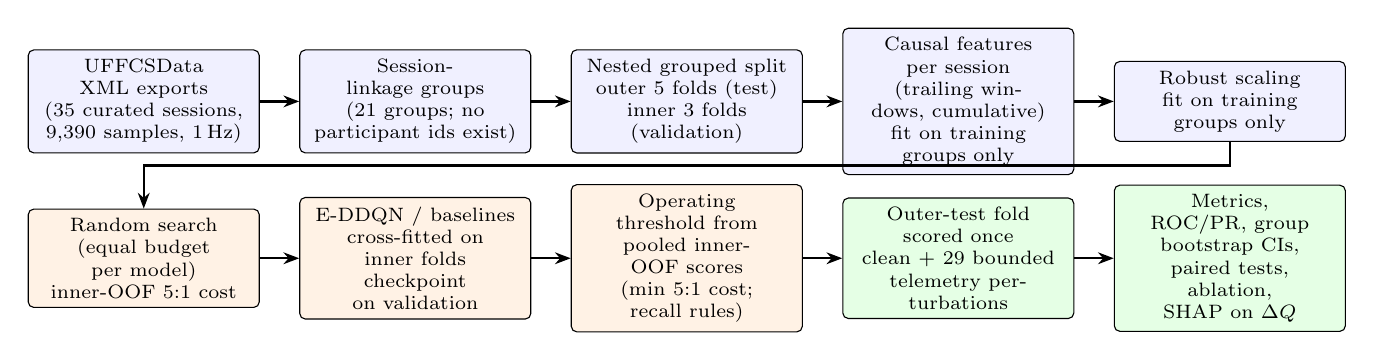
\begin{tikzpicture}[
  node distance=4mm and 5mm,
  box/.style={draw, rounded corners=2pt, align=center, font=\scriptsize, minimum height=9mm, text width=27mm, fill=#1},
  box/.default=white,
  arr/.style={-{Stealth[length=2mm]}, thick}]
\node[box=blue!6] (raw) {UFFCSData XML exports\\(\nSessionsEval{} curated sessions,\\ \nSamplesEval{} samples, 1\,Hz)};
\node[box=blue!6, right=of raw] (grp) {Session-linkage groups\\(\nGroupsEval{} groups; no\\participant ids exist)};
\node[box=blue!6, right=of grp] (split) {Nested grouped split\\outer \nOuter{} folds (test)\\inner \nInner{} folds (validation)};
\node[box=blue!6, right=of split] (feat) {Causal features per session\\(trailing windows, cumulative)\\fit on training groups only};
\node[box=blue!6, right=of feat] (scale) {Robust scaling\\fit on training groups only};
\node[box=orange!10, below=7mm of raw] (hpo) {Random search\\(equal budget per model)\\inner-OOF 5:1 cost};
\node[box=orange!10, right=of hpo] (train) {E-DDQN / baselines\\cross-fitted on inner folds\\checkpoint on validation};
\node[box=orange!10, right=of train] (thr) {Operating threshold from\\pooled inner-OOF scores\\(min 5:1 cost; recall rules)};
\node[box=green!10, right=of thr] (test) {Outer-test fold scored once\\clean + 29 bounded\\telemetry perturbations};
\node[box=green!10, right=of test] (stats) {Metrics, ROC/PR, group\\bootstrap CIs, paired tests,\\ablation, SHAP on $\Delta Q$};
\draw[arr] (raw) -- (grp);
\draw[arr] (grp) -- (split);
\draw[arr] (split) -- (feat);
\draw[arr] (feat) -- (scale);
\draw[arr] (scale.south) |- ++(0,-3mm) -| (hpo.north);
\draw[arr] (hpo) -- (train);
\draw[arr] (train) -- (thr);
\draw[arr] (thr) -- (test);
\draw[arr] (test) -- (stats);
\end{tikzpicture}
\caption{Revised, leakage-free pipeline. Blue: data construction (no step looks across a partition boundary); orange: model development using inner (validation) folds only; green: single evaluation of each outer-test fold with the frozen protocol.}
\label{fig:pipeline}
\end{figure*}

\subsection{Data Source, Provenance and Target}
\label{sec:data}
The experiments use UFFCSData~\cite{porcino2019uffcsdata,porcino2022identifying,porcino2021methodology}, a public dataset in which volunteers played a race game and a flight game in a head-mounted display while the game logged, about once per second, the player's speed and acceleration, the camera orientation (quaternion components), the frame rate, the region of interest, session-configuration flags and the participant's self-reported discomfort level on a 0--3 scale; a Cybersickness Profile Questionnaire (CSPQ: gender, age band, VR experience, glasses, vision problems, eye dominance, flicker sensitivity) is stored with every session. The submitted version of this paper called these data ``GLCD'' and used a derived file whose preprocessing history could not be verified; we rebuilt everything from the original XML exports. The dataset authors' curated release (\nSessionsEval{} seated sessions recorded in December~2019; \nSamplesEval{} samples) is identical, sample by sample, to \nSessionsEval{} of the raw exports and is our evaluation set. The \nSessionsDev{} standing-posture sessions recorded in October~2019 are used \emph{only} to debug code and calibrate training budgets; two further raw sessions that the dataset authors excluded are not used.

The binary target is unchanged from the submitted version: $y_t=1$ (\emph{cybersickness event}) if the reported discomfort level at second $t$ is at least~1, and $y_t=0$ otherwise. The prevalence is \prevEval{} (Flight \prevFlight{}, Race \prevRace{}). We stress that $y$ marks self-reported discomfort, \emph{not} the presence of an attack: no session in the dataset was attacked. In the submitted version, every minority grade had been oversampled to the size of grade~0 (5,243 samples) \emph{before} a random row-level split; this created duplicated samples across training and test partitions and an artificial 3:1 class ratio (Section~\ref{sec:leak}).

\subsection{Unit of Independence and Splits}
\label{sec:groups}
The release contains no participant identifier, and sessions are not independent: some participants restarted after an aborted session (e.g., a 104-s session followed 108\,s later by a full session with an identical nine-field CSPQ profile). We therefore form conservative \emph{session-linkage groups}: sessions are linked if their CSPQ profiles are identical, or if a session follows an aborted one ($<200$ samples) within 180\,s with at most two differing questionnaire fields; connected components are groups. This yields \nGroupsEval{} groups. The rule may merge different people who share a profile---which only makes evaluation more conservative---but it cannot reveal one person who answered the questionnaire differently in non-consecutive sessions; we report this residual risk as a limitation.

All splits are made at the group level. A nested design is used: \nOuter{} outer folds (stratified by game and label) provide test data, and within each outer development set \nInner{} inner grouped folds provide validation data for hyper-parameter search, checkpoint selection and threshold selection. Every sample of the evaluation set is therefore predicted exactly once, by models that never saw its session, its linkage group or its exact questionnaire profile. Executable checks confirm zero session, group and profile overlap and zero duplicated feature rows between any development set and its test fold.

\subsection{Causal Feature Engineering and Preprocessing}
\label{sec:features}
Features of second $t$ use only seconds $0,\dots,t$ of the same session (verified by recomputing features on sessions truncated at random $t$). They comprise the game indicator, elapsed time, instantaneous speed, acceleration and $|$acceleration$|$, the camera quaternion components, the per-second orientation change $\lVert q_t-q_{t-1}\rVert$, the frame rate (the logger writes 0 on the very first sample of some sessions; this artefact is imputed with the training median), the region of interest, trailing-window (5\,s and 15\,s) means, standard deviations, deltas, maxima, minima, acceleration-spike rates and frame-drop fractions, and cumulative exposure descriptors (cumulative orientation change, spike and frame-drop counts, running mean speed); 39 telemetry features in total, plus 14 CSPQ indicators. The spike threshold (90th percentile of $|$acceleration$|$) and the imputation value are learned on training rows only; the frame-drop threshold (80\,fps, i.e. $>11\%$ below the 90-Hz target) is fixed. Features are scaled with a median/IQR scaler fitted on training rows. Constant or redundant columns were removed: the field of view, the static-frame and auto-camera flags are constant within each game (pure game indicators), four configuration flags and posture are constant overall, and the absolute player position was excluded because it encodes elapsed course distance and is absent in the October wave. Which of four feature sets a model uses---\emph{telemetry}, \emph{telemetry+profile}, a small a-priori \emph{exposure} set (game, elapsed time, cumulative orientation change, cumulative spikes, running and 15-s mean speed, 15-s mean rotation rate and $|$acceleration$|$), or \emph{exposure+profile}---is a hyper-parameter chosen on validation folds. No oversampling or synthetic data are used anywhere; class imbalance is handled only inside training.

\subsection{Decision Formulation: MDP or Contextual Bandit?}
\label{sec:formulation}
Following the submitted version, detection is cast as a sequential decision process over each recorded session (an \emph{episode}). The state $s_t\in\mathbb{R}^d$ is the causal feature vector at second $t$; the action $a_t\in\{0,1\}$ is \emph{stay silent} or \emph{raise an alarm}; the reward is $r_t=R(a_t,y_t)$ with
\begin{equation}
R(1,1)=+0.5,\ R(0,0)=+0.1,\ R(0,1)=-0.5,\ R(1,0)=-0.1;
\label{eq:reward}
\end{equation}
the next state $s_{t+1}$ is the next second \emph{of the same session}, and the last sample of a session is terminal. No transition ever links two sessions.

Because the telemetry was logged while participants played, without any alarm in the loop, the action cannot influence later observations: $P(s_{t+1}\mid s_t,a_t)=P(s_{t+1}\mid s_t)$. For any discount $\gamma<1$ the optimal action-value function then decomposes as
\begin{equation}
Q^*(s,a)=\mathbb{E}[R(a,y)\mid s]+\gamma\,\mathbb{E}[V^*(s_{t+1})\mid s_t=s],
\label{eq:decomp}
\end{equation}
whose second term does not depend on $a$. Hence (i) the optimal policy is myopic for every $\gamma$, i.e. the logged-data problem is a \emph{contextual bandit}~\cite{lattimore2020bandit} rather than a control problem in which actions steer future states; and (ii) with $p(s)=P(y=1\mid s)$,
\begin{equation}
Q^*(s,1)-Q^*(s,0)=p(s)\,\Delta_{\mathrm{FN}}-(1-p(s))\,\Delta_{\mathrm{FP}},
\label{eq:margin}
\end{equation}
with regrets $\Delta_{\mathrm{FN}}=R(1,1)-R(0,1)=1.0$ and $\Delta_{\mathrm{FP}}=R(0,0)-R(1,0)=0.2$. The greedy policy alarms iff $p(s)\ge \Delta_{\mathrm{FP}}/(\Delta_{\mathrm{FN}}+\Delta_{\mathrm{FP}})=1/6$, which is exactly the Bayes-optimal decision of a cost-sensitive classifier with misclassification costs $C_{\mathrm{FN}}:C_{\mathrm{FP}}=5:1$~\cite{elkan2001cost}. The asymmetric reward is therefore not a different objective from cost-sensitive learning: it encodes the same 5:1 operating point. Bootstrapping with $\gamma>0$ adds an action-independent term whose estimation noise enters both Q-values; it cannot improve the optimal policy and helps or hurts only through estimation effects. We therefore treat $\gamma\in\{0,0.5,0.9,0.99\}$ as a hyper-parameter selected on validation data and also evaluate the $\gamma=0$ special case as a separately tuned model (E-CB). A genuine MDP would require the alarm to change future rendering or symptoms (e.g., a mitigation in the loop); no such intervention exists in the data, so we make no claim that E-DDQN learns adaptive sequential control. Equation~\eqref{eq:margin} also gives every Q-learner a calibrated-probability scale, $\hat p(s)=(\Delta Q+\Delta_{\mathrm{FP}})/(\Delta_{\mathrm{FN}}+\Delta_{\mathrm{FP}})$, used to place all models on a common score scale.

\subsection{E-DDQN (Corrected)}
\label{sec:eddqn}
E-DDQN keeps the components of the submitted design, with the defects found during the audit removed.
\emph{Network.} A multilayer trunk (width and depth tuned) with batch or layer normalisation~\cite{ioffe2015bn}, ReLU and dropout~\cite{srivastava2014dropout} feeds a dueling head~\cite{wang2016dueling}, $Q(s,a)=V(s)+A(s,a)-\frac{1}{2}\sum_{a'}A(s,a')$, with raw (unsquashed) Q-values.
\emph{Target.} The Double-DQN target~\cite{vanhasselt2016double} with terminal flags,
\begin{equation}
y_t=r_t+\gamma(1-d_t)\,Q_{\theta^-}\big(s_{t+1},\arg\max_{a'}Q_\theta(s_{t+1},a')\big),
\end{equation}
where the online arg-max is computed in evaluation mode, and the Huber loss~\cite{girshick2015fast} is minimised with Adam~\cite{kingma2015adam}, weight decay, gradient clipping at 1.0 and a cosine learning-rate schedule~\cite{loshchilov2017sgdr}.
\emph{Target network.} Polyak averaging $\theta^-\leftarrow(1-\tau)\theta^-+\tau\theta$~\cite{lillicrap2016continuous} after every update; the batch-normalisation running statistics are copied as well (the submitted code averaged parameters only, so the target network normalised with mean~0 and variance~1 forever).
\emph{Replay.} A circular buffer~\cite{lin1992selfimproving} from which minibatches are drawn with a fixed class composition $\rho$ (Normal) and $1-\rho$ (event).
\emph{Exploration and warm-up.} $\varepsilon$-greedy exploration decaying per epoch from 1.0 to 0.01; optional warm-up with uniformly random actions.
\emph{No teacher forcing.} The submitted code computed the reward of a random action but stored the \emph{true label} as the action (e.g., a random ``silent'' decision on an event was stored as \emph{alarm} with reward $-0.5$), training the correct action toward the false-negative penalty. This procedure is removed. Because labels are available offline, the reward of \emph{both} actions is known; E-DDQN may instead store the counterfactual action together with \emph{its own} reward (\emph{full-information replay}), a valid transition that turns Q-learning into cost-sensitive regression of $\mathbb{E}[R\mid s,a]$. Whether to use it is tuned.
\emph{Checkpointing.} Every second epoch the agent is scored on the inner validation groups; the epoch with the lowest achievable 5:1 cost (ties: higher PR-AUC) is kept.
Algorithm~\ref{alg:eddqn} summarises training. Executable unit tests verify the 5:1 regret ratio, within-session transitions with one terminal per session, reward/action consistency of every stored transition, target-network buffer synchronisation and bounded Q-values.

\begin{algorithm}[t]
\caption{Corrected E-DDQN training for one inner split}
\label{alg:eddqn}
\begin{algorithmic}[1]
\small
\State Initialise $\theta$, $\theta^-\!\leftarrow\theta$, buffer $\mathcal{D}$; optional warm-up with random actions on within-session transitions
\For{epoch $=1,\dots,E$}
  \State Concatenate training sessions in random order, each in temporal order; mark the last second of each session terminal
  \For{each chunk of 256 consecutive transitions}
    \State $a_t\gets$ $\varepsilon$-greedy on $Q_\theta(s_t,\cdot)$;\ $r_t\gets R(a_t,y_t)$
    \State store $(s_t,a_t,r_t,s_{t+1},d_t,y_t)$; if full-information replay, also store $(s_t,1-a_t,R(1-a_t,y_t),s_{t+1},d_t,y_t)$
    \State every 2 chunks: $k$ updates on class-balanced minibatches (Double-DQN target, Huber loss); Polyak update of $\theta^-$ and copy of BN statistics
  \EndFor
  \State 5 consolidation updates;\ decay $\varepsilon$;\ cosine LR step
  \State every 2 epochs: score inner-validation groups; keep $\theta$ if the achievable 5:1 cost improves
\EndFor
\State \Return checkpoint; score $\hat p(s)=(\Delta Q+\Delta_{\mathrm{FP}})/(\Delta_{\mathrm{FN}}+\Delta_{\mathrm{FP}})$
\end{algorithmic}
\end{algorithm}

\subsection{Matched Baselines}
\label{sec:baselines}
All models receive the same splits, the same four candidate feature sets, the same binary target, the same random-search budget (16 configurations; 12 for logistic regression), the same checkpoint rule (neural models), the same cross-fitted training recipe and the same threshold rules. \textbf{Standard DQN}~\cite{mnih2015human}: symmetric $\pm1$ reward, single max-operator target, periodic hard target copies (every 10, 100 or 500 updates), uniform replay, plain (non-dueling) head, same episodes and transitions; $\gamma$ is tuned as for E-DDQN. \textbf{E-CB}: E-DDQN with $\gamma=0$ (contextual bandit; the target network and double estimator are then inactive by construction). \textbf{CS-MLP}: a cost-sensitive multilayer perceptron with the same trunk family and a positive-class-weighted cross-entropy ($w=5$, i.e. the same 5:1 cost), uniform or class-balanced minibatches, checkpointed like the agents. \textbf{Logistic regression}, \textbf{histogram gradient boosting} and \textbf{random forest}~\cite{pedregosa2011sklearn} with class weight 5. For a weighted model the output $p_w$ is mapped back to $\hat p=p_w/(5-4p_w)$, so that every model's score estimates $P(y=1\mid s)$ and the Bayes cut-off is $1/6$ for all of them. Two trivial references are reported: \emph{always alarm} and \emph{never alarm}.

\subsection{Threat Model and Telemetry-Perturbation Stress Tests}
\label{sec:threat}
The motivating threat is unchanged: an adversary who controls the rendering or locomotion pipeline (e.g., a malicious modification or compromised runtime) degrades frame pacing~\cite{odeleye2021framerate}, distorts camera or locomotion motion, or manipulates the field of view to induce or exploit cybersickness~\cite{tseng2022dark,kundu2025securing}. The dataset contains \emph{no attacked sessions} and no measurement of what any manipulation would do to a participant. We therefore evaluate only what the data support: \emph{synthetic, bounded perturbations of the logged telemetry channels} of the outer-test sessions, after which the causal features are recomputed with the frozen, training-fitted featurizer---exactly as a deployed monitor would see manipulated telemetry. Labels are never changed; an indicator $z$ marks perturbed seconds. Scenarios (frozen before evaluation): \emph{frame-rate capping} to 72/60/45\,fps (Type~I); \emph{camera-orientation jitter} $\pm0.02/0.05/0.10$ per quaternion component (Type~II); \emph{speed up-scaling} by 10/25/50\,\% with acceleration recomputed (Type~II); \emph{acceleration-spike injection} of 10/20/40 units every 20\,s (Type~II); each over the whole session or a random 60-s window, all clipped to the ranges observed in the data. \emph{Field-of-view manipulation (Type~III) is not evaluated} because the field of view never varies in the data (it is constant within each game), so any perturbation would be pure extrapolation. Two adversarial goals are analysed with a per-session worst case over the whole-session candidates plus three ``hiding'' manipulations (speed down-scaling, orientation smoothing, frame-rate restoration): \emph{evasion} (minimise alarms on event seconds; the adversary is given the labels) and \emph{false-alarm induction} (maximise alarms on non-event seconds). These are feature-space stress tests of the detector; they are not demonstrations of physical rendering attacks.

\subsection{Evaluation Protocol and Statistics}
\label{sec:protocol}
The protocol was written and committed before any model was trained on the evaluation sessions. For every model family and outer fold, random search draws the family's configurations; each is trained on each inner split and the configuration with the lowest 5:1 expected cost on the pooled inner out-of-fold (OOF) predictions (at the cost-minimising threshold; ties broken by PR-AUC) is selected. The selected configuration is then trained for five seeds; for each seed the \nInner{} inner models are kept (each checkpointed on its own validation groups), the outer-test score is the mean of their scores, and the operating threshold is chosen on the pooled inner-OOF scores of the development groups only. The primary operating rule (D1) minimises the 5:1 expected cost $c=(5\,\mathrm{FN}+\mathrm{FP})/N$ on those OOF scores; secondary rules are the untuned Bayes cut-off $\hat p\ge1/6$ (D0; for the asymmetric agents this is the greedy arg-max policy) and a validation recall constraint of 0.95. Matched operating points use validation-chosen thresholds for recall targets 0.80--0.99 and specificity targets 0.5 and 0.8. The outer-test folds are never used for any choice.

We report accuracy, precision, recall, specificity, F1, balanced accuracy, MCC~\cite{chicco2020mcc}, G-mean, false-positive and false-negative rates, missed events, the 5:1 expected cost, ROC-AUC and PR-AUC~\cite{saito2015pr}, exact confusion matrices, mean~$\pm$~SD over the five seeds, and 95\,\% confidence intervals from a bootstrap that resamples linkage groups (2,000 replicates). Paired comparisons use the same test samples: McNemar's test~\cite{mcnemar1947,dietterich1998tests} (exact binomial and continuity-corrected $\chi^2$; the contingency table is checked against the error counts, $b-c=\mathrm{err}_B-\mathrm{err}_A$) and a paired group bootstrap of the cost difference. Because consecutive seconds of a session are strongly dependent, the sample-level McNemar test overstates the evidence; the group bootstrap is the primary inference. Event-level metrics (sessions whose event is detected, detection delay after onset, alarm fraction before onset and in event-free sessions) complement the per-second metrics.

\subsection{Explainability}
\label{sec:shap}
SHAP values~\cite{lundberg2017shap} are computed with DeepExplainer~\cite{shrikumar2017deeplift} for the decision margin $\Delta Q(s)=Q(s,1)-Q(s,0)$ of E-DDQN (one model per outer fold, background drawn from that fold's training groups, attributions on its test groups). The submitted version attributed $Q(s,\textit{Attack})$, which contains the state value $V(s)$ shared by both actions and therefore does not explain the decision.

\section{Experimental Setup}
\label{sec:setup}

\subsection{Implementation}
All models are implemented in PyTorch~\cite{paszke2019pytorch} and scikit-learn~\cite{pedregosa2011sklearn} and run on CPU with one thread per process. The data parser, grouping, causal features, agents, baselines, perturbation generator, protocol runner and statistics are in \texttt{revision/src} and \texttt{revision/scripts}; \texttt{run\_all.sh} regenerates every number in this paper from the raw XML files.

\subsection{Search Spaces and Budgets}
The search spaces (Supplementary Table~S3) are shared wherever a hyper-parameter is common to several families. Neural models: feature set (four options), trunk (64--64, 128--128, 256--256 or 256--512--256), dropout (0--0.3), normalisation (batch or layer), learning rate ($3\times10^{-4}$--$3\times10^{-3}$), weight decay (0--$10^{-3}$) and batch size (256 or 512). Agents additionally: $\varepsilon$ decay per epoch (0.90--0.97), warm-up (0 or 4,000 random-action transitions) and updates per learning step (1, 2 or 4); E-DDQN: $\gamma\in\{0,0.5,0.9,0.99\}$, $\tau\in\{0.005,0.01,0.05\}$, replay composition $\rho\in\{0.4,0.5,0.6\}$ and full-information replay (on/off); E-CB: $\rho$ and full-information replay; DQN: $\gamma$ and the hard-update period (10, 100 or 500 updates); CS-MLP: uniform or class-balanced minibatches. All agents are trained for 40 epochs (one epoch is one pass over every training session in temporal order), with chunks of 256 transitions, a learning step every two chunks, five consolidation updates per epoch, a 50,000-transition buffer and gradient clipping at 1.0; the CS-MLP is trained for 40 epochs. Validation-based checkpoints are taken every two epochs. These budgets were calibrated on the October-2019 development-only sessions, where validation cost plateaued after 20--30 epochs. Each family receives \HPOBudget{} random configurations (12 for logistic regression), drawn once with a fixed seed and evaluated on every inner split of every outer fold. Gradient boosting and random forests search learning rate, number of iterations, leaf counts, minimum leaf sizes, $\ell_2$ regularisation, depth and feature sub-sampling; logistic regression searches the inverse regularisation strength $C\in[10^{-4},10]$. The configuration selected for each outer fold is listed in Supplementary Table~S4.

\subsection{Seeds and Repetitions}
Final models are trained with five seeds per outer fold; for every seed the outer-test score is the average of the \nInner{} cross-fitted inner models. We report mean~$\pm$~SD over seeds and, for paired tests and confidence intervals, the \emph{seed ensemble} (the mean score over the five seeds, with its threshold chosen on the mean OOF score). No seed was selected or discarded.

\subsection{Leakage Audit of the Submitted Protocol}
To quantify the effect of the submitted data pipeline, we reconstructed it from \texttt{dataset.csv}: every grade was randomly oversampled to 5,243 samples and the result split 70/15/15 at row level, which reproduces the submitted partition sizes (14,680 / 3,146 / 3,146) exactly. The same 21 raw columns were then evaluated (i) under this protocol, (ii) under a row-level split without oversampling, and (iii) under the grouped split of Section~\ref{sec:groups}, with an untuned gradient-boosting classifier; the unmodified submitted E-DDQN script was also run on the reconstructed partition and on a grouped partition. Because the submitted 41-feature files are not available, this is a proxy reproduction.

\section{Results}
\label{sec:results}

\subsection{The Submitted Results Are Explained by Data Leakage}
\label{sec:leak}
Table~\ref{tab:leak} reproduces the submitted protocol. Oversampling every discomfort grade to 5,243 samples before a 70/15/15 row split reproduces the submitted partition sizes exactly, and an untuned gradient-boosting classifier then reaches \LeakOldAcc\,\% accuracy, \LeakOldRecall\,\% recall and MCC \LeakOldMCC{}---numbers as high as those reported for E-DDQN in the submitted version, obtained without any reinforcement learning. Under that protocol \LeakDupPos{} of the \LeakTestPos{} positive test rows (\LeakDupPct\,\%) have an exact duplicate in the training split, and every session contributes to both splits. The unmodified submitted E-DDQN script behaves the same way: \OrigOldRecall\,\% recall and MCC \OrigOldMCC{} on the reconstructed partition, but MCC \OrigGrpMCC{} once the split respects session-linkage groups. With the same columns and a grouped split, gradient boosting falls to ROC-AUC \LeakGrpRocAuc{} (MCC \LeakGrpMCC{}). The published numbers therefore measure the ability to recognise duplicated and temporally adjacent samples of sessions seen during training, not the ability to detect cybersickness in new sessions. All results below use the leakage-free protocol of Section~\ref{sec:protocol}.

\begin{table*}[t]
\centering
\caption{Effect of the evaluation protocol on the same data (21 raw columns of the curated release). Test-split metrics; ``proxy'' marks the reconstruction of the submitted pipeline (its 41-feature files were not available).}
\label{tab:leak}
\resizebox{\textwidth}{!}{\begin{tabular}{llccccc}
\toprule
Model & Evaluation protocol & Acc. & Recall & Spec. & MCC & ROC-AUC \\
\midrule
HGB & Oversample to 5,243/grade, then 70/15/15 row split (submitted protocol) & 97.6 & 99.8 & 91.0 & 0.935 & 0.995 \\
HGB & Row-level random split, no oversampling & 95.3 & 94.1 & 96.3 & 0.905 & 0.992 \\
HGB & Grouped 5-fold split (session-linkage groups) & 52.2 & 33.6 & 66.9 & 0.005 & 0.523 \\
E-DDQN (submitted code) & Submitted script, submitted protocol (proxy) & 95.2 & 99.2 & 83.1 & 0.870 & -- \\
E-DDQN (submitted code) & Submitted script, grouped split (proxy) & 41.1 & 92.1 & 7.7 & $-$0.004 & -- \\
\bottomrule
\end{tabular}
}
\end{table*}

\subsection{Leakage-Free Comparison under the 5:1 Cost}
\label{sec:main}
Table~\ref{tab:main} reports the primary analysis: every model tuned, checkpointed and thresholded on validation groups only and scored once on the outer-test groups (all \nSamplesEval{} samples, \nSessionsEval{} sessions). Two facts dominate. First, the detection problem is hard once sessions and participants are not shared: the best ranking performance is ROC-AUC \HGBCostRocAucMean{} (HGB) and \RFCostRocAucMean{} (random forest), and the highest mean PR-AUC is \DQNCostPrAucMean{} (DQN) against a prevalence of 0.44. Second, under a 5:1 cost the cost-minimising operating point of every model lies close to ``always alarm'' (cost \AlwaysCost): validation-selected thresholds yield recall of 93--99\,\% but specificity of only 3--18\,\%. Only the random forest improves materially on the trivial policy (cost \RFCostCostMean$\pm$\RFCostCostSD{} vs.\ \AlwaysCost), and even its group-bootstrap 95\,\% CI (seed ensemble, \RFCICostLo--\RFCICostHi) includes the always-alarm cost; logistic regression (\LRCostCostMean) and gradient boosting (\HGBCostCostMean) improve on it only marginally.

The corrected E-DDQN ranks last of the \nModels{} models on the primary rule: recall \EDDQNCostRecallMean$\pm$\EDDQNCostRecallSD\,\%, specificity \EDDQNCostSpecMean$\pm$\EDDQNCostSpecSD\,\%, cost \EDDQNCostCostMean$\pm$\EDDQNCostCostSD{} (worse than always alarming), ROC-AUC \EDDQNCostRocAucMean$\pm$\EDDQNCostRocAucSD{} and MCC \EDDQNCostMCCMean. The standard DQN baseline reaches cost \DQNCostCostMean{} and ROC-AUC \DQNCostRocAucMean, and the contextual-bandit variant E-CB cost \ECBCostCostMean{} and ROC-AUC \ECBCostRocAucMean. Neither RL model beats the cost of always alarming. E-DDQN therefore does \emph{not} improve on the standard DQN in this controlled comparison; the improvement reported in the submitted version does not survive leakage-free evaluation.

\begin{table*}[t]
\centering
\caption{Primary analysis (rule D1: threshold minimising the 5:1 cost on pooled inner-validation predictions). Mean~$\pm$~SD over five seeds of the pooled outer-test metrics (\nSamplesEval{} samples; recall, specificity, precision, F1 and balanced accuracy in \%); FN and FP are exact counts of the seed ensemble. Bold: lowest cost. HGB and logistic regression are deterministic given the data, hence SD = 0.}
\label{tab:main}
\resizebox{\textwidth}{!}{\begin{tabular}{lccccccccccc}
\toprule
Model & Recall & Spec. & Prec. & F1 & Bal. acc. & MCC & Cost$_{5:1}$ & ROC-AUC & PR-AUC & FN & FP \\
\midrule
\textbf{E-DDQN} & 93.4$\pm$2.5 & 7.4$\pm$2.7 & 44.4$\pm$0.7 & 60.2$\pm$0.9 & 50.4$\pm$1.2 & 0.016$\pm$0.054 & 0.663$\pm$0.048 & 0.538$\pm$0.016 & 0.483$\pm$0.019 & 400 & 4,820 \\
E-CB & 97.1$\pm$2.9 & 8.4$\pm$2.8 & 45.6$\pm$0.6 & 62.1$\pm$1.0 & 52.8$\pm$1.2 & 0.122$\pm$0.052 & 0.575$\pm$0.055 & 0.653$\pm$0.011 & 0.562$\pm$0.006 & 140 & 4,480 \\
DQN & 95.2$\pm$2.7 & 14.5$\pm$4.9 & 46.8$\pm$1.0 & 62.8$\pm$0.8 & 54.8$\pm$1.6 & 0.158$\pm$0.038 & 0.584$\pm$0.040 & 0.661$\pm$0.013 & 0.595$\pm$0.022 & 129 & 4,391 \\
CS-MLP & 99.4$\pm$0.7 & 2.8$\pm$1.9 & 44.7$\pm$0.4 & 61.7$\pm$0.4 & 51.1$\pm$0.8 & 0.072$\pm$0.049 & 0.557$\pm$0.012 & 0.644$\pm$0.018 & 0.521$\pm$0.022 & 23 & 4,925 \\
LogReg & 99.1$\pm$0.0 & 8.1$\pm$0.0 & 46.0$\pm$0.0 & 62.9$\pm$0.0 & 53.6$\pm$0.0 & 0.167$\pm$0.000 & 0.532$\pm$0.000 & 0.626$\pm$0.000 & 0.576$\pm$0.000 & 36 & 4,817 \\
HGB & 97.0$\pm$0.0 & 14.6$\pm$0.0 & 47.3$\pm$0.0 & 63.6$\pm$0.0 & 55.8$\pm$0.0 & 0.197$\pm$0.000 & 0.543$\pm$0.000 & 0.692$\pm$0.000 & 0.593$\pm$0.000 & 124 & 4,479 \\
RF & 98.5$\pm$0.3 & 18.2$\pm$0.7 & 48.8$\pm$0.2 & 65.2$\pm$0.1 & 58.3$\pm$0.3 & 0.266$\pm$0.004 & \textbf{0.491$\pm$0.003} & 0.688$\pm$0.002 & 0.548$\pm$0.001 & 54 & 4,281 \\
\midrule
Always alarm & 100.0 & 0.0 & 44.2 & 61.3 & 50.0 & 0.000 & 0.558 & -- & -- & 0 & 5,243 \\
Never alarm & 0.0 & 100.0 & -- & -- & 50.0 & 0.000 & 2.208 & -- & -- & 4,147 & 0 \\
\bottomrule
\end{tabular}
}
\end{table*}

\begin{figure}[t]
\centering
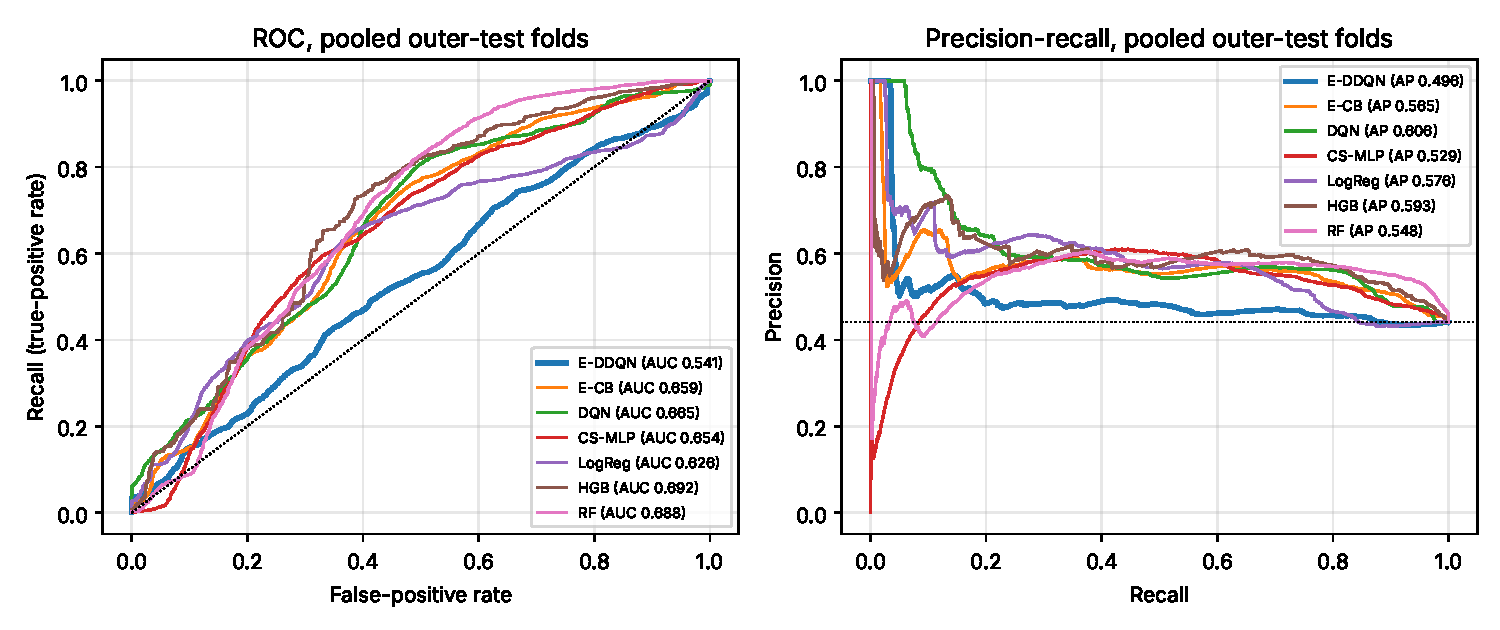
\includegraphics[width=\columnwidth]{figs/roc_pr_main.pdf}
\caption{ROC and precision--recall curves of the seed-ensemble scores, pooled over the five outer-test folds.}
\label{fig:rocpr}
\end{figure}

\subsection{Operating Points, Matched Recall and the Asymmetric Reward}
\label{sec:op}
Table~\ref{tab:ops} contrasts three operating rules. With the untuned Bayes cut-off $\hat p\ge 1/6$ (rule D0)---for the asymmetric agents this is simply the greedy policy $\arg\max_a Q(s,a)$---E-DDQN obtains recall \EDDQNBayesRecallMean\,\% at specificity \EDDQNBayesSpecMean\,\% (cost \EDDQNBayesCostMean), whereas the random forest obtains recall \RFBayesRecallMean\,\% at specificity \RFBayesSpecMean\,\% (cost \RFBayesCostMean). When every model is held to a validation recall of at least 0.95, the random forest again has the lowest cost (\RFRecCostMean; E-DDQN \EDDQNRecCostMean). At validation-matched recall targets (Table~\ref{tab:matched}), the thresholds transfer worst for E-DDQN: at both recall targets it attains lower test recall than every supervised model, and at the 0.95 target it also has a higher false-positive rate than all of them. Reading the ROC curves at fixed recall (descriptive only), the false-positive rate at 95\,\% recall is \EDDQNRocFPRatNineFive\,\% for E-DDQN and \RFRocFPRatNineFive\,\% for the random forest. Because the reward encodes the same 5:1 operating point as a cost-weighted classifier (Eq.~\eqref{eq:margin}), the asymmetric reward provides no advantage that cost-weighted training plus a validation-selected threshold does not already provide.

\begin{table}[t]
\centering
\caption{Expected 5:1 cost (mean over seeds) under three operating rules chosen without test data.}
\label{tab:ops}
\footnotesize
\begin{tabular}{lccc}
\toprule
Model & D1: min cost & D0: $\hat p\ge 1/6$ & val.\ recall $\ge$ 0.95 \\
\midrule
E-DDQN & \EDDQNCostCostMean & \EDDQNBayesCostMean & \EDDQNRecCostMean \\
E-CB & \ECBCostCostMean & \ECBBayesCostMean & \ECBRecCostMean \\
DQN & \DQNCostCostMean & \DQNBayesCostMean & \DQNRecCostMean \\
CS-MLP & \CSMLPCostCostMean & \CSMLPBayesCostMean & \CSMLPRecCostMean \\
LogReg & \LRCostCostMean & \LRBayesCostMean & \LRRecCostMean \\
HGB & \HGBCostCostMean & \HGBBayesCostMean & \HGBRecCostMean \\
RF & \RFCostCostMean & \RFBayesCostMean & \RFRecCostMean \\
\midrule
Always alarm & \AlwaysCost & \AlwaysCost & \AlwaysCost \\
\bottomrule
\end{tabular}
\end{table}

\begin{table*}[t]
\centering
\caption{Matched operating points: thresholds chosen on validation predictions to reach the stated recall or specificity; test recall (\%), false-positive rate (\%) and false-positive count of the seed ensemble.}
\label{tab:matched}
\resizebox{\textwidth}{!}{\begin{tabular}{lccccccccc}
\toprule
 & \multicolumn{3}{c}{val. recall $\ge$ 0.90} & \multicolumn{3}{c}{val. recall $\ge$ 0.95} & \multicolumn{3}{c}{val. specificity $\ge$ 0.80} \\
Model & Rec. & FPR & FP & Rec. & FPR & FP & Rec. & FPR & FP \\
\midrule
E-DDQN & 81.7 & 77.0 & 4,036 & 84.5 & 86.6 & 4,539 & 25.2 & 18.6 & 974 \\
E-CB & 88.6 & 68.0 & 3,565 & 92.4 & 78.1 & 4,093 & 31.2 & 17.4 & 910 \\
DQN & 88.0 & 64.2 & 3,366 & 91.7 & 72.7 & 3,810 & 32.2 & 14.2 & 743 \\
CS-MLP & 94.1 & 78.4 & 4,111 & 97.5 & 85.1 & 4,463 & 24.2 & 12.7 & 666 \\
LogReg & 92.8 & 73.5 & 3,856 & 97.2 & 81.7 & 4,285 & 37.7 & 22.5 & 1,181 \\
HGB & 95.4 & 72.2 & 3,785 & 97.5 & 81.7 & 4,282 & 24.3 & 11.3 & 594 \\
RF & 93.7 & 64.0 & 3,358 & 96.9 & 74.3 & 3,896 & 21.0 & 13.3 & 695 \\
\bottomrule
\end{tabular}
}
\end{table*}

\subsection{Statistical Comparison}
\label{sec:stats}
Table~\ref{tab:paired} compares E-DDQN with every other model on identical test samples (seed ensembles, rule D1). For every pair the McNemar contingency table satisfies $b-c=\mathrm{err}_B-\mathrm{err}_A$ (checked programmatically and recomputed with an independent library). Sample-level McNemar tests give $p<0.001$ for every pair, but they treat \nSamplesEval{} strongly autocorrelated seconds as independent and overstate the evidence. The group bootstrap, which resamples the \nGroupsEval{} independent units, shows that E-DDQN's cost is higher than that of the random forest by \PairDOneRFCostDiff{} (95\,\% CI \PairDOneRFCostLo{} to \PairDOneRFCostHi; $p=$\,\PairDOneRFPboot), higher than gradient boosting by \PairDOneHGBCostDiff{} ($p=$\,\PairDOneHGBPboot), logistic regression by \PairDOneLRCostDiff{} ($p=$\,\PairDOneLRPboot), CS-MLP by \PairDOneCSMLPCostDiff{} ($p=$\,\PairDOneCSMLPPboot) and E-CB by \PairDOneECBCostDiff{} ($p=$\,\PairDOneECBPboot); the difference from the standard DQN (\PairDOneDQNCostDiff; $p=$\,\PairDOneDQNPboot) is not significant at the 5\,\% level. Group-bootstrap confidence intervals of every model are given in Supplementary Sec.~S3.2; with only \nGroupsEval{} independent groups they are wide.

\begin{table*}[t]
\centering
\caption{Paired comparisons with E-DDQN (A) on the same \nSamplesEval{} test samples (seed ensembles, rule D1). $b$: A correct, B wrong; $c$: A wrong, B correct. $\Delta$Cost and its CI and $p_{\text{group}}$ come from 2,000 group-bootstrap replicates; $p_{\text{exact}}$ is the sample-level exact McNemar test.}
\label{tab:paired}
\resizebox{\textwidth}{!}{\begin{tabular}{lcccccccc}
\toprule
B (vs. A = E-DDQN) & $b$ & $c$ & err$_A$ & err$_B$ & $\chi^2_{cc}$ & $p_{\text{exact}}$ & $\Delta$Cost$_{5:1}$ (A$-$B) [95\% CI] & $p_{\text{group}}$ \\
\midrule
E-CB & 299 & 899 & 5,220 & 4,620 & 299.5 & $<$0.001 & +0.175 [+0.016, +0.448] & 0.014 \\
DQN & 297 & 997 & 5,220 & 4,520 & 377.6 & $<$0.001 & +0.190 [$-$0.017, +0.493] & 0.079 \\
CS-MLP & 402 & 674 & 5,220 & 4,948 & 68.3 & $<$0.001 & +0.190 [+0.005, +0.485] & 0.039 \\
LogReg & 389 & 756 & 5,220 & 4,853 & 117.0 & $<$0.001 & +0.194 [+0.011, +0.477] & 0.026 \\
HGB & 203 & 820 & 5,220 & 4,603 & 370.9 & $<$0.001 & +0.183 [+0.011, +0.460] & 0.035 \\
RF & 293 & 1,178 & 5,220 & 4,335 & 531.2 & $<$0.001 & +0.242 [+0.052, +0.528] & 0.001 \\
\bottomrule
\end{tabular}
}
\end{table*}

\subsection{Event-Level Behaviour}
At the cost-optimal operating points every model flags almost every session: E-DDQN raises an alarm on \EDDQNEvFreeAlarm\,\% of the seconds of the \nEventFreeSessions{} sessions in which no discomfort was ever reported and on \EDDQNEvPreAlarm\,\% of the seconds before onset in the \nEventSessions{} sessions with an event (random forest: \RFEvFreeAlarm\,\% and \RFEvPreAlarm\,\%). Events are therefore ``detected'' with zero median delay by construction, not through discrimination (Supplementary Sec.~S3.4).

\subsection{Why E-DDQN Under-Performs: Bootstrapping and Selection Optimism}
\label{sec:why}
Validation selected $\gamma=$ \EDDQNGammas{} for the five outer folds of E-DDQN, i.e.\ strong bootstrapping, and the exposure+profile feature set in \EDDQNnProfile{} of 5 folds. Section~\ref{sec:formulation} shows that bootstrapping cannot improve the optimal policy here and adds action-independent estimation noise to $\Delta Q$. Two diagnostics agree. (i) The separately tuned $\gamma=0$ variant (E-CB) ranks much better (ROC-AUC \ECBCostRocAucMean{} vs.\ \EDDQNCostRocAucMean). (ii) Table~\ref{tab:optimism} compares, per family, the inner-validation cost of the configuration at the moment it was selected with its outer-test cost. The gap is \EDDQNOptGap{} for E-DDQN but between \RFOptGap{} and \ECBOptGap{} for all other models: noisy, high-variance training curves combined with validation checkpointing and selection let E-DDQN configurations look best on validation folds by chance~\cite{varma2006bias}. Q-value estimates stay finite---the largest magnitudes over all runs (E-DDQN \EDDQNQAbsMax, DQN \DQNQAbsMax, E-CB \ECBQAbsMax) slightly exceed the corresponding return bounds $r_{\max}/(1-\gamma)$ in a few runs, i.e.\ extrapolation on atypical states---so the failure is not numerical divergence; the mean greedy-action Q-value differs from its realised discounted validation return by \EDDQNOverest{} for E-DDQN, \DQNOverest{} for DQN and \ECBOverest{} for E-CB (Supplementary Sec.~S3.6).

\begin{table}[t]
\centering
\caption{Selection optimism: pooled inner-validation 5:1 cost of the selected configuration (HPO seed) versus its outer-test cost (mean over folds and seeds).}
\label{tab:optimism}
\resizebox{\columnwidth}{!}{\begin{tabular}{lccc}
\toprule
Model & Inner-OOF cost at selection & Outer-test cost & Gap \\
\midrule
E-DDQN & 0.467 & 0.754 & +0.288 \\
E-CB & 0.488 & 0.557 & +0.070 \\
DQN & 0.478 & 0.544 & +0.065 \\
CS-MLP & 0.501 & 0.534 & +0.033 \\
LogReg & 0.518 & 0.531 & +0.014 \\
HGB & 0.518 & 0.539 & +0.021 \\
RF & 0.495 & 0.481 & $-$0.015 \\
\bottomrule
\end{tabular}
}
\end{table}

\subsection{Component Ablation and Reward-Ratio Sensitivity}
\label{sec:ablation}
Table~\ref{tab:ablation} removes or changes one component of E-DDQN at a time while keeping the configuration selected for each outer fold fixed (five seeds; same protocol). Every variant ranks close to chance (ROC-AUC \AblSoftCostRocAuc--\AblGammaZeroCostRocAuc). No single change moves the cost by more than about one seed standard deviation of the full model (\EDDQNCostCostMean$\pm$\EDDQNCostCostSD). The lowest cost is obtained by \emph{replacing} the asymmetric reward with the symmetric $\pm1$ reward (\AblAsymCostCost) and the highest ROC-AUC by switching off bootstrapping ($\gamma=0$; \AblGammaZeroCostRocAuc); hard target copies (\AblSoftCostCost), no dueling head (\AblDuelCostCost), uniform replay (\AblBalCostCost), no warm-up (\AblWarmCostCost) and toggling full-information replay (\AblFullCostCost) leave the cost essentially unchanged, and removing the double estimator slightly increases it (\AblDoubleCostCost). In contrast to the ablation of the submitted version, none of these components can be credited with a gain in safety or accuracy. Every variant is scored on the same implied-probability scale and thresholded with the same rules, so the reward table can act only through the learned scores; at the fixed cut-off $\hat p\ge1/6$ (rule D0) the symmetric-reward variant is not worse either (cost \AblAsymBayesCost{} vs.\ \EDDQNBayesCostMean).

\begin{table}[t]
\centering
\caption{Leave-one-component-out ablation of E-DDQN (selected configuration per outer fold held fixed; rule D1; mean over 5 seeds, cost $\pm$ SD).}
\label{tab:ablation}
\resizebox{\columnwidth}{!}{\begin{tabular}{lccccc}
\toprule
Variant & Recall & Spec. & Cost$_{5:1}$ & ROC-AUC & PR-AUC \\
\midrule
Full E-DDQN (selected) & 93.4 & 7.4 & 0.663$\pm$0.048 & 0.538 & 0.483 \\
\midrule
full-information replay toggled & 93.7 & 5.4 & 0.667$\pm$0.106 & 0.563 & 0.500 \\
symmetric $\pm$1 reward instead of asymmetric & 94.8 & 8.6 & 0.625$\pm$0.038 & 0.572 & 0.517 \\
uniform instead of class-balanced replay & 94.3 & 4.3 & 0.660$\pm$0.045 & 0.554 & 0.486 \\
no double estimator (max-operator target) & 93.1 & 5.3 & 0.681$\pm$0.086 & 0.543 & 0.491 \\
no dueling head & 94.6 & 5.8 & 0.644$\pm$0.059 & 0.559 & 0.494 \\
hard target copy every 10 updates & 94.9 & 6.5 & 0.634$\pm$0.043 & 0.529 & 0.472 \\
no warm-up & 93.8 & 7.1 & 0.656$\pm$0.049 & 0.547 & 0.497 \\
$\gamma=0$ (contextual bandit) & 94.4 & 6.4 & 0.645$\pm$0.070 & 0.576 & 0.510 \\
\bottomrule
\end{tabular}
}
\end{table}

Table~\ref{tab:ratio} varies the false-negative to false-positive regret of the reward from 1:1 to 10:1 (E-DDQN configuration per fold fixed; ratio 5:1 reproduces the main E-DDQN run bit for bit, which also confirms the determinism of the pipeline). The greedy policy moves along the trade-off exactly as Eq.~\eqref{eq:margin} predicts: recall rises from \RatioArgOneRecall\,\% (1:1) to \RatioArgFiveRecall\,\% (5:1) and \RatioArgOneZeroRecall\,\% (10:1), while specificity falls from \RatioArgOneSpec\,\% to \RatioArgFiveSpec\,\% and \RatioArgOneZeroSpec\,\%. Once the threshold is chosen on validation data, however, all ratios end at statistically indistinguishable costs (\RatioTunedOneCost--\RatioTunedOneZeroCost) and similar ranking: the reward ratio sets the default operating point, but it does not create discrimination that a threshold cannot reproduce. The 5:1 ratio is therefore best understood as a declared safety preference whose operating point can equally be reached by cost-weighted training or threshold selection.

\begin{table*}[t]
\centering
\caption{Reward-ratio sensitivity of E-DDQN: operating point of the greedy (arg-max) policy, whose implied cut-off on $P(y=1\mid s)$ is $1/(1+R)$, and of the validation-tuned threshold (rule D1). Mean ($\pm$ SD) over five seeds.}
\label{tab:ratio}
\footnotesize
\input{generated/tab_ratio_policy.tex}
\end{table*}



\subsection{Robustness under Telemetry Perturbations}
\label{sec:attack}
Table~\ref{tab:attack-auc} reports threshold-free ranking performance under each frozen perturbation. \AttAucFracSmall\,\% of the model--scenario combinations change the pooled ROC-AUC by less than 0.03 and none by more than \AttAucMaxAbsChange{} (the largest drops occur for acceleration-spike injection in E-CB and DQN and for speed down-scaling in gradient boosting), and several perturbations even raise it slightly: the detectors depend only weakly on the frame-rate, orientation and locomotion channels, mainly because the dominant inputs selected on validation data are exposure time, cumulative exposure and questionnaire answers. At the cost-optimal operating points (Table~\ref{tab:attack}), the per-session worst-case evasion adversary lowers recall on event seconds from \EDDQNAttCleanRecall\,\% to \EDDQNAttWorstRecall\,\% for E-DDQN, from \ECBAttCleanRecall\,\% to \ECBAttWorstRecall\,\% for E-CB and from \RFAttCleanRecall\,\% to \RFAttWorstRecall\,\% for the random forest, while the false-alarm adversary drives the false-positive rate of every model to \EDDQNAttWorstFPR--100\,\% (it is already \RFAttCleanFPR--\CSMLPAttCleanFPR\,\% without attack). These are feature-space stress tests: they show how far bounded manipulation of the logged channels can move the detectors' decisions, not what a real rendering attack would do to a participant, and they cannot evaluate field-of-view manipulation, which never varies in the data.

\begin{table*}[t]
\centering
\caption{Threshold-free robustness: pooled outer-test ROC-AUC of the seed-ensemble score on clean telemetry and under whole-session perturbations (the last column gives the most negative and most positive change over all 21 whole-session variants).}
\label{tab:attack-auc}
\resizebox{\textwidth}{!}{\begin{tabular}{lcccccccc}
\toprule
Model & Clean & fps$\le$45 & jitter 0.10 & speed $\times$1.5 & spikes 40 & speed $\times$0.5 & smooth 0.25 & min / max $\Delta$ \\
\midrule
E-DDQN & 0.541 & 0.541 & 0.593 & 0.561 & 0.559 & 0.532 & 0.539 & $-$0.008 / +0.053 \\
E-CB & 0.659 & 0.659 & 0.682 & 0.648 & 0.575 & 0.648 & 0.658 & $-$0.089 / +0.052 \\
DQN & 0.665 & 0.665 & 0.677 & 0.680 & 0.605 & 0.632 & 0.676 & $-$0.064 / +0.035 \\
CS-MLP & 0.654 & 0.649 & 0.654 & 0.630 & 0.652 & 0.629 & 0.646 & $-$0.025 / +0.005 \\
LogReg & 0.626 & 0.677 & 0.639 & 0.620 & 0.629 & 0.608 & 0.639 & $-$0.017 / +0.051 \\
HGB & 0.692 & 0.694 & 0.709 & 0.650 & 0.698 & 0.647 & 0.712 & $-$0.068 / +0.019 \\
RF & 0.688 & 0.689 & 0.708 & 0.667 & 0.683 & 0.723 & 0.725 & $-$0.021 / +0.037 \\
\bottomrule
\end{tabular}
}
\end{table*}

\begin{table*}[t]
\centering
\caption{Recall/false-positive rate (\%) on perturbed seconds at the D1 operating point, and per-session adaptive worst cases (evasion: minimum recall; false-alarm induction: maximum FPR) over all whole-session candidates.}
\label{tab:attack}
\resizebox{\textwidth}{!}{\begin{tabular}{lcccccccc}
\toprule
 & Clean & fps$\le$45 & jitter 0.10 & speed $\times$1.5 & spikes 40 & \multicolumn{2}{c}{Adaptive worst case} \\
Model & Rec./FPR & Rec./FPR & Rec./FPR & Rec./FPR & Rec./FPR & Rec. (evasion) & FPR (false alarm) \\
\midrule
E-DDQN & 90.4/91.9 & 90.4/91.9 & 94.0/92.2 & 93.5/90.7 & 95.4/94.3 & 82.9 & 94.5 \\
E-CB & 96.6/85.4 & 96.6/85.4 & 96.1/88.2 & 98.7/95.9 & 99.3/97.7 & 78.0 & 98.9 \\
DQN & 96.9/83.7 & 96.9/83.7 & 94.8/83.5 & 97.8/91.8 & 97.9/95.4 & 87.3 & 97.5 \\
CS-MLP & 99.4/93.9 & 100.0/98.3 & 99.7/96.5 & 100.0/98.2 & 99.9/99.1 & 95.6 & 100.0 \\
LogReg & 99.1/91.9 & 97.0/86.3 & 99.2/92.7 & 99.7/94.9 & 99.9/96.7 & 95.4 & 96.7 \\
HGB & 97.0/85.4 & 97.0/85.9 & 96.3/82.7 & 98.2/91.7 & 98.1/95.7 & 81.0 & 96.1 \\
RF & 98.7/81.7 & 98.7/81.3 & 98.0/81.1 & 99.0/92.1 & 99.8/97.4 & 90.5 & 98.4 \\
\bottomrule
\end{tabular}
}
\end{table*}

\subsection{Explainability}
\label{sec:xai}
SHAP attributions of the E-DDQN decision margin $\Delta Q$ (Fig.~\ref{fig:shap}) are dominated by \ShapTopFive{}. The detector's decisions are driven mainly by exposure time, cumulative exposure and questionnaire answers rather than by instantaneous telemetry, which is consistent with its insensitivity to the telemetry perturbations above. Because attributions are computed after the decision, they add no latency to detection.

\begin{figure}[t]
\centering
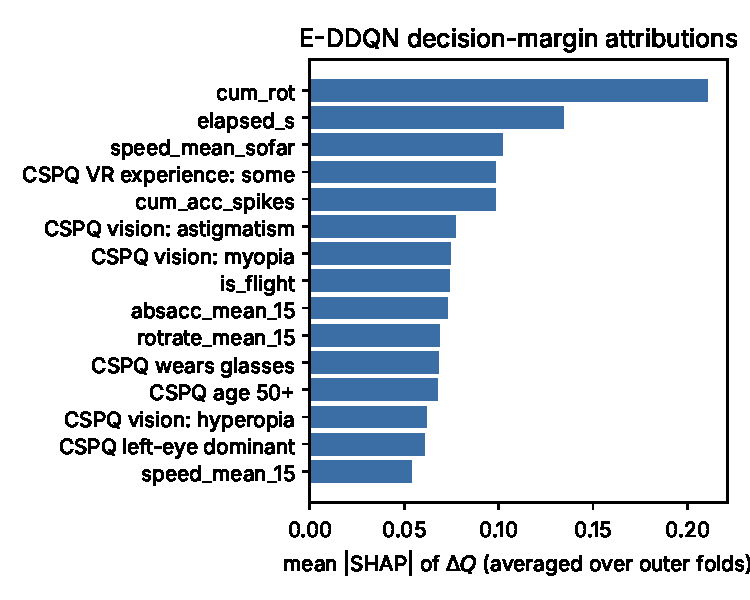
\includegraphics[width=0.92\columnwidth]{figs/shap_margin.pdf}
\caption{Mean absolute SHAP value of the E-DDQN decision margin $\Delta Q$, averaged over the five outer folds (one model per fold; attributions on that fold's test groups).}
\label{fig:shap}
\end{figure}

\section{Discussion}
\label{sec:discussion}

\subsection{What Changed Relative to the Submitted Version}
The submitted version reported 96.88\,\% accuracy and 99.53\,\% recall for E-DDQN and a large gain over a standard DQN. Section~\ref{sec:leak} shows that numbers of that size follow from the data pipeline---oversampling before a row-level split, so that duplicated and temporally adjacent samples of the same sessions appear in training and test---and are reproduced by a generic classifier without reinforcement learning. Under a participant-conservative, nested and frozen protocol, the same data support only modest discrimination (best ROC-AUC \RFCostRocAucMean--\HGBCostRocAucMean), the corrected E-DDQN does not outperform the standard DQN, and the best cost-sensitive decision rule comes from a random forest. We have therefore replaced every numerical claim of the submitted version and withdrawn the claim that E-DDQN improves accuracy, recall, F1 and MCC over a standard DQN.

\subsection{Is E-DDQN Reinforcement Learning?}
With logged data the alarm cannot influence the subsequent telemetry, so the decision problem is a contextual bandit (Section~\ref{sec:formulation}). E-DDQN remains a valid value-based learner of a cost-sensitive detection policy, and its episodes, transitions and terminal states are now defined consistently with the data. However, (i) the asymmetric reward is mathematically equivalent to a 5:1 cost-sensitive Bayes threshold, so it is a statement about the operating point rather than a different learning objective; (ii) bootstrapping cannot improve the optimal policy, and empirically strong bootstrapping ($\gamma$ close to 1) made the learned margins noisy and the validation-based selection over-optimistic; and (iii) under bandit feedback the agent observes the reward of one action only, although labels reveal both, which is why full-information replay (storing each counterfactual action with its own reward) is the principled replacement for teacher forcing. Adaptive sequential control would require an intervention in the loop---for example an alarm that triggers a rendering mitigation whose effect on later telemetry and symptoms is measured---which no public cybersickness dataset provides.

\subsection{The Safety Objective}
A 5:1 cost makes an alarm the cheaper decision whenever $P(y=1\mid s)\ge1/6$. With a prevalence of 0.44 and weakly informative inputs, almost every second satisfies this, so the cost-optimal policy of every model is close to ``always alarm'': recall is high, but \DOneFPRMin--\DOneFPRMax\,\% of non-event seconds also trigger an alarm (mean over seeds, rule D1). High recall alone is therefore not evidence of a useful safety monitor, and the comparison has to be made on cost, specificity at matched recall and threshold-free ranking. On those criteria the intended safety objective---near-complete detection with a controlled false-alarm rate---is \emph{not} achieved by any model on these data. The obstacle is the information content of game telemetry: once participants are not shared between training and test, exposure time, accumulated motion and the pre-session questionnaire carry most of the usable signal, and they distinguish individual susceptibility only coarsely.

\subsection{The Adversarial Threat Model}
The threat model is motivated by documented attacks on VR perception and frame pacing~\cite{odeleye2021framerate,tseng2022dark,kundu2025securing}, but UFFCSData contains no attacked sessions, so the binary target is a cybersickness label, not an attack label. What the data support is a stress test of the detector under bounded manipulation of the frame-rate, orientation and locomotion channels; field-of-view manipulation cannot be tested because the field of view never varies in the data. Under these tests, \AttAucFracSmall\,\% of model--scenario combinations change ROC-AUC by less than 0.03 and none by more than \AttAucMaxAbsChange, because the detectors rely mostly on exposure and questionnaire inputs, whereas an adaptive adversary who knows the labels can lower recall on event seconds by \AttEvasionDropMin--\AttEvasionDropMax{} percentage points, depending on the model. Demonstrating detection of real rendering attacks requires data in which manipulations are applied to participants under ethical approval and their physiological effects are measured.

\subsection{Limitations}
(i) A single public dataset with \nSessionsEval{} curated sessions and \nGroupsEval{} independent groups; confidence intervals are wide and fold-to-fold variation is large. (ii) Participant identity cannot be verified; linkage groups are conservative but cannot exclude a participant who answered the questionnaire differently in non-consecutive sessions. (iii) The label is a coarse self-report sampled at 1\,Hz and is nearly monotone within a session. (iv) Perturbations are synthetic and feature-space; their physiological effect is unknown. (v) Hyper-parameter search used an identical but modest budget (\HPOBudget{} configurations per family); a larger budget could change the ranking of the neural models, although the selection-optimism analysis suggests that additional search would mostly increase optimism. (vi) The October-2019 sessions were used only for development and could not serve as an external test set because their camera-orientation channels were not logged.

\subsection{Implications}
Accuracies reported on gameplay cybersickness datasets---including ours in the submitted version---should be read together with the split protocol: with 1-Hz samples and near-monotone labels, any split that shares sessions or participants between training and test inflates performance to near-perfect levels. For safety-prioritised detection, the asymmetric reward should be treated as what it is, a cost-sensitive operating point, and RL detectors should be compared with cost-weighted supervised models at matched recall or cost under participant-independent evaluation.

\section{Conclusion}
\label{sec:conclusion}
This revision re-examined E-DDQN, a dueling Double DQN with an asymmetric (5:1) reward, class-balanced replay and soft target updates, for safety-prioritised cybersickness detection motivated by an adversarial threat model, and compared it with a standard DQN and with cost-sensitive supervised models. Rebuilding the pipeline from the original UFFCSData exports revealed that the previously reported performance was produced by oversampling before a row-level split; with the same data and a grouped split, performance falls to near chance for the original columns. We corrected the E-DDQN implementation (valid within-session transitions with terminal flags, removal of an invalid teacher-forcing scheme, target-network normalisation statistics), proved that on logged data the problem is a contextual bandit whose asymmetric-reward optimum equals the 5:1 cost-sensitive Bayes threshold, and evaluated all models under one frozen, nested, participant-conservative protocol. Under that protocol E-DDQN reached cost \EDDQNCostCostMean{} and ROC-AUC \EDDQNCostRocAucMean, did not outperform the standard DQN (cost \DQNCostCostMean, ROC-AUC \DQNCostRocAucMean), and was significantly worse than a cost-weighted random forest (cost \RFCostCostMean, ROC-AUC \RFCostRocAucMean); only the random forest improved materially on always alarming (cost \AlwaysCost), and with \nGroupsEval{} independent groups even that improvement is not statistically established. Bounded telemetry perturbations changed threshold-free performance by at most \AttAucMaxAbsChange{} ROC-AUC, while adaptive worst-case manipulation reduced recall on event seconds. The safety objective of near-complete detection with controlled false alarms is not achieved on these data. Future work requires datasets with physiological or eye-tracking signals, verified participant identifiers and, for the adversarial claim, manipulations applied to participants with measured effects.


\section*{Data Availability and Reproducibility}
The data are the publicly available UFFCSData release~\cite{porcino2019uffcsdata} (AGPL-3.0). All code, the frozen protocol (\texttt{revision/\allowbreak configs/\allowbreak protocol.json}, committed before any model was trained on the evaluation sessions), the split tables, the per-sample predictions of every model and every script that produces the numbers, tables and figures of this paper are in the project repository (\texttt{revision/\allowbreak }); \texttt{revision/\allowbreak run\_all.sh} regenerates everything from the raw XML files. Seeds are fixed for data splitting (20261012), hyper-parameter search (777) and final training (1000--1004); CPU execution with one thread per process was used, and minor floating-point differences across hardware are possible.

\section*{Acknowledgment}
The authors thank Universiti Teknologi PETRONAS for institutional and computational support, and the authors of the UFFCSData dataset for making their data public.

\section*{Conflict of Interest}
The authors declare no conflict of interest.

\section*{Funding}
This research received no specific grant from any funding agency in the public, commercial, or not-for-profit sectors.

\bibliographystyle{IEEEtran}
\bibliography{refs}

\end{document}
